%\VignetteIndexEntry{genAriseGUI Vignette}
%\VignetteDepends{}
%\VignetteKeywords{microarray analyzer GUI}
%\VignettePackage{genAriseGUI}
\documentclass[12pt]{article}
\topmargin=0in
\oddsidemargin 0.0in
\evensidemargin 0.0in
\usepackage{url}
\usepackage{Sweave}
\usepackage{graphicx}
\usepackage{fancyhdr}
\pagestyle{fancy}
\headheight 35pt 
\fancyhead[R]{\Large{\bf{genArise}}} %Especifico

\title{The genArise Package}
\author{Ana Patricia G\'omez May\'en\\ Gustavo Corral Guill\'e\\ Lina Riego Ruiz\\ Gerardo Coello Couti\~no}

\begin{document}

\maketitle

\section{Introduction}

genArise is a package that contains specific functions to perform an analysis of microarray obtained data to select genes that are significantly differentially expressed between classes of samples. Before this analysis, genArise carry out a number of transformations on the data to eliminate low-quality measurements and to adjust the measured intensities to facilitate comparisons.\\

First, you must install the R system. The current released version is 2.0.0 and the binary can be obtained via CRAN, a collection of sites which carry identical material, consisting of the R distribution(s), the contributed extensions, documentation for R, and binaries. The CRAN master site can be found at the URL \url{http://cran.R-project.org/}. \\

Then, you need install the packages tkrplot and locfit in order to be able to use this package. This can be done as follows:
\begin{Scode}
> install.packages(c("locfit","tkrplot"))
\end{Scode}

Finally, genArise can be loaded with the next instruction:\\
\begin{Schunk}
\begin{Sinput}
> library(genArise)
\end{Sinput}
\begin{Soutput}
Loading required package: locfit 
Locfit for R.
August 3, 2000.  (Updated for R 1.7.0, March 21, 2003)

Attaching package 'locfit':


	The following object(s) are masked from package:stats :

	 knots 

Loading required package: tkrplot 
Loading required package: tcltk 
\end{Soutput}
\end{Schunk}
Once loaded, you can proceed with the analysis of the microarray data. genArise is provided with functions that can be applied from R prompt in every step of analysis; however, there is also a graphical user interface to facilitate the use of all the functions in the package.

\section{The genArise Package's Functions}
The first step that you must do is to read the data contained in the input file.\\

To read the input files genArise have the function \texttt{read.spot}. This function returns an object of type Spot, because a number of functions that carry out transformations on the data need a spot object as argument. The syntax for this function is:

\begin{Scode}
> my.spot <- read.spot( file.name, cy3 = 1, cy5 = 2, 
  bg.cy3 = 3, bg.cy5 = 4, ids = 5, header = FALSE, 
  sep = "\t", is.ifc = FALSE)	
\end{Scode}

\begin{Soutput}
Output: an object of class Spot called my.spot
\end{Soutput}

And the meaning of each one of the arguments is:\\

\begin{description}
\item{file.name:} this is the name of the file which the data are to be read from.  The input file format must be in columns of data which values are separated by some character. The default separator is tab character, but you can change that in the sep argument of this function. The input file must contain a row for each spot in the grid, at least that the experiment was performed by the IFC in UNAM (the 13 last rows contain statistical information about the experiment) and probably a header row.
\item{cy3:} location of the column that contain the query sample in the array (red color).
\item{cy5:} location of the column that contain the reference sample in the array (green color).
\item{bg.cy3:} location of the column that contain the background correction for cy3.
\item{bg.cy5:} location of the column that contain the background correction for cy5.
\item{ids:} location of the column that contain the ids for the distinct elements in the array.
\item{header:} a logical value indicating whether the file contains the names of the variables as its first row.
\item{sep:} the field separator character.  Values on each line of the file are separated by this character.
\item{is.ifc:} a logical value indicating whether the experiment was performed by the Microarray Unit of the Cellular Physiology Institute of UNAM. It just eliminate the last 13 rows that contain a statistic about the experiment.
\end{description}

As an example for describing each package's function contained in this user's manual we will use a subset of the microarray data object generated with \texttt{read.spot} function. This subset is called Simon and it can be loaded in this way:

\begin{Schunk}
\begin{Sinput}
> data(Simon)
> ls()
\end{Sinput}
\begin{Soutput}
[1] "Simon"
\end{Soutput}
\end{Schunk}

\begin{Soutput}
You have created an object of the class Spot in the current
environment so you will be able to apply to that object any 
function of genArise that receives a spot as argument.
\end{Soutput}

\subsection{Diagnostic plots}
Previous to any kind of analysis, once you have load the input, you are able to visualize it using the function \texttt{imageLimma}. This function constructs an image plot in a green to red scale representing the $log_2$ intensity ratio for each spot on the array. See Figure \ref{fig1}. The imageLimma function receives several arguments depending on the data that is going to be analyzed.\footnote{imageLimma is completly based in the imageplot function from the limma package.\\ \textit{Gordon K. Smyth (2004) \textquotedblleft Linear Models and Empirical Bayes Methods for Assessing Differential Expression in Microarray Experiments \textquotedblright, Statistical Applications in Genetics and Molecular Biology: Vol. 3: No. 1, Article 3. \url{http://www.bepress.com/sagmb/vol3/iss1/art3}}} \\

\begin{figure}[h]
\begin{center}
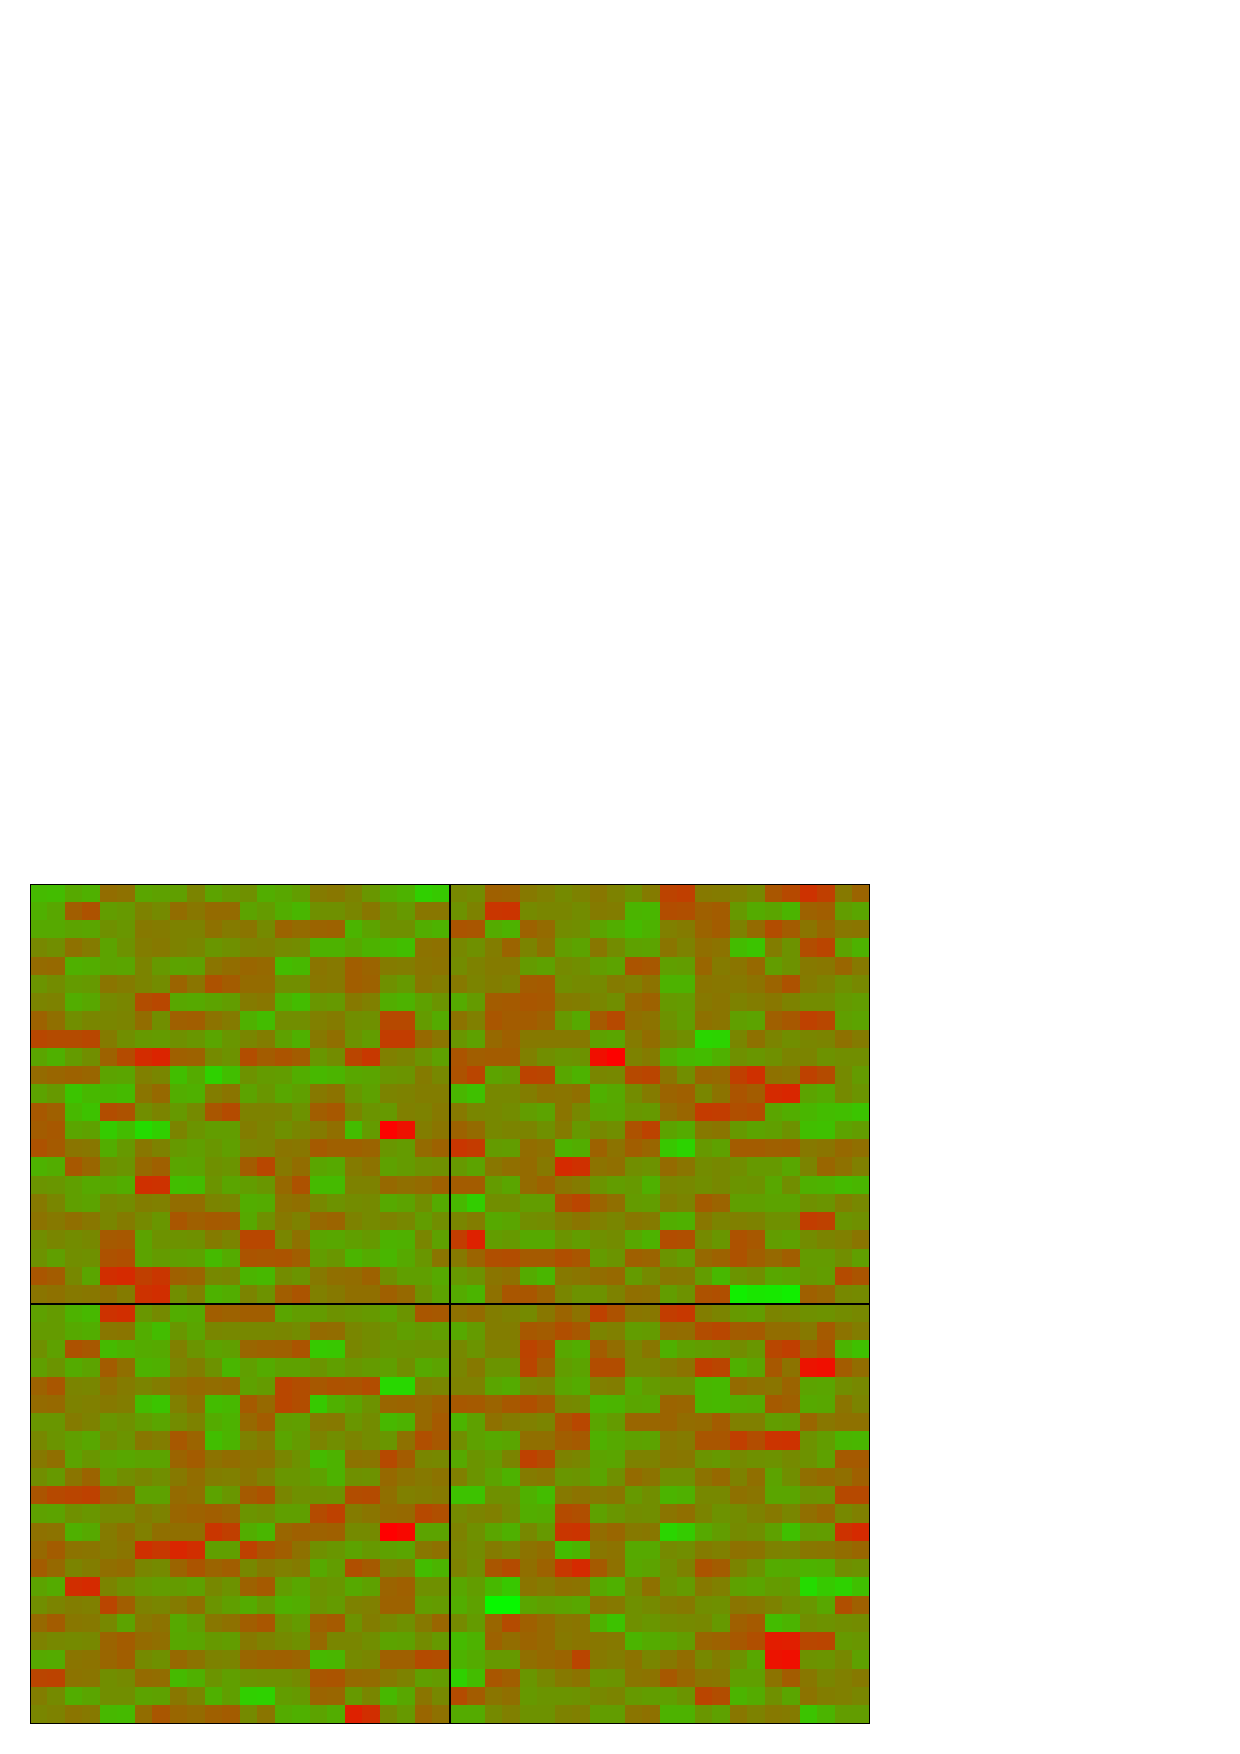
\includegraphics{example-genArise-003}
\caption{Image plot in a green to red scale.\label{fig1}}
\end{center}
\end{figure}
\begin{Scode}
> data(Simon)
> datos <- attr(Simon, "spotData")# Extract spot data
> M <- log(datos$Cy3, 2) - log(datos$Cy5, 2)
> imageLimma(z = M, row = 23, column = 24, meta.row = 2, 
  meta.column = 2, low = NULL, high = NULL)
\end{Scode}

\begin{Soutput}
Output: Plot the intensity values
\end{Soutput}

In the same way that you can plot the $log_2$ intensity ratio for each spot, you can also plot the background value that correspond to each one of the intensities. See Figure \ref{fig2} and \ref{fig3}.\\

For example, this is the plot for Cy3 intensities.
\begin{figure}[h]
\begin{center}
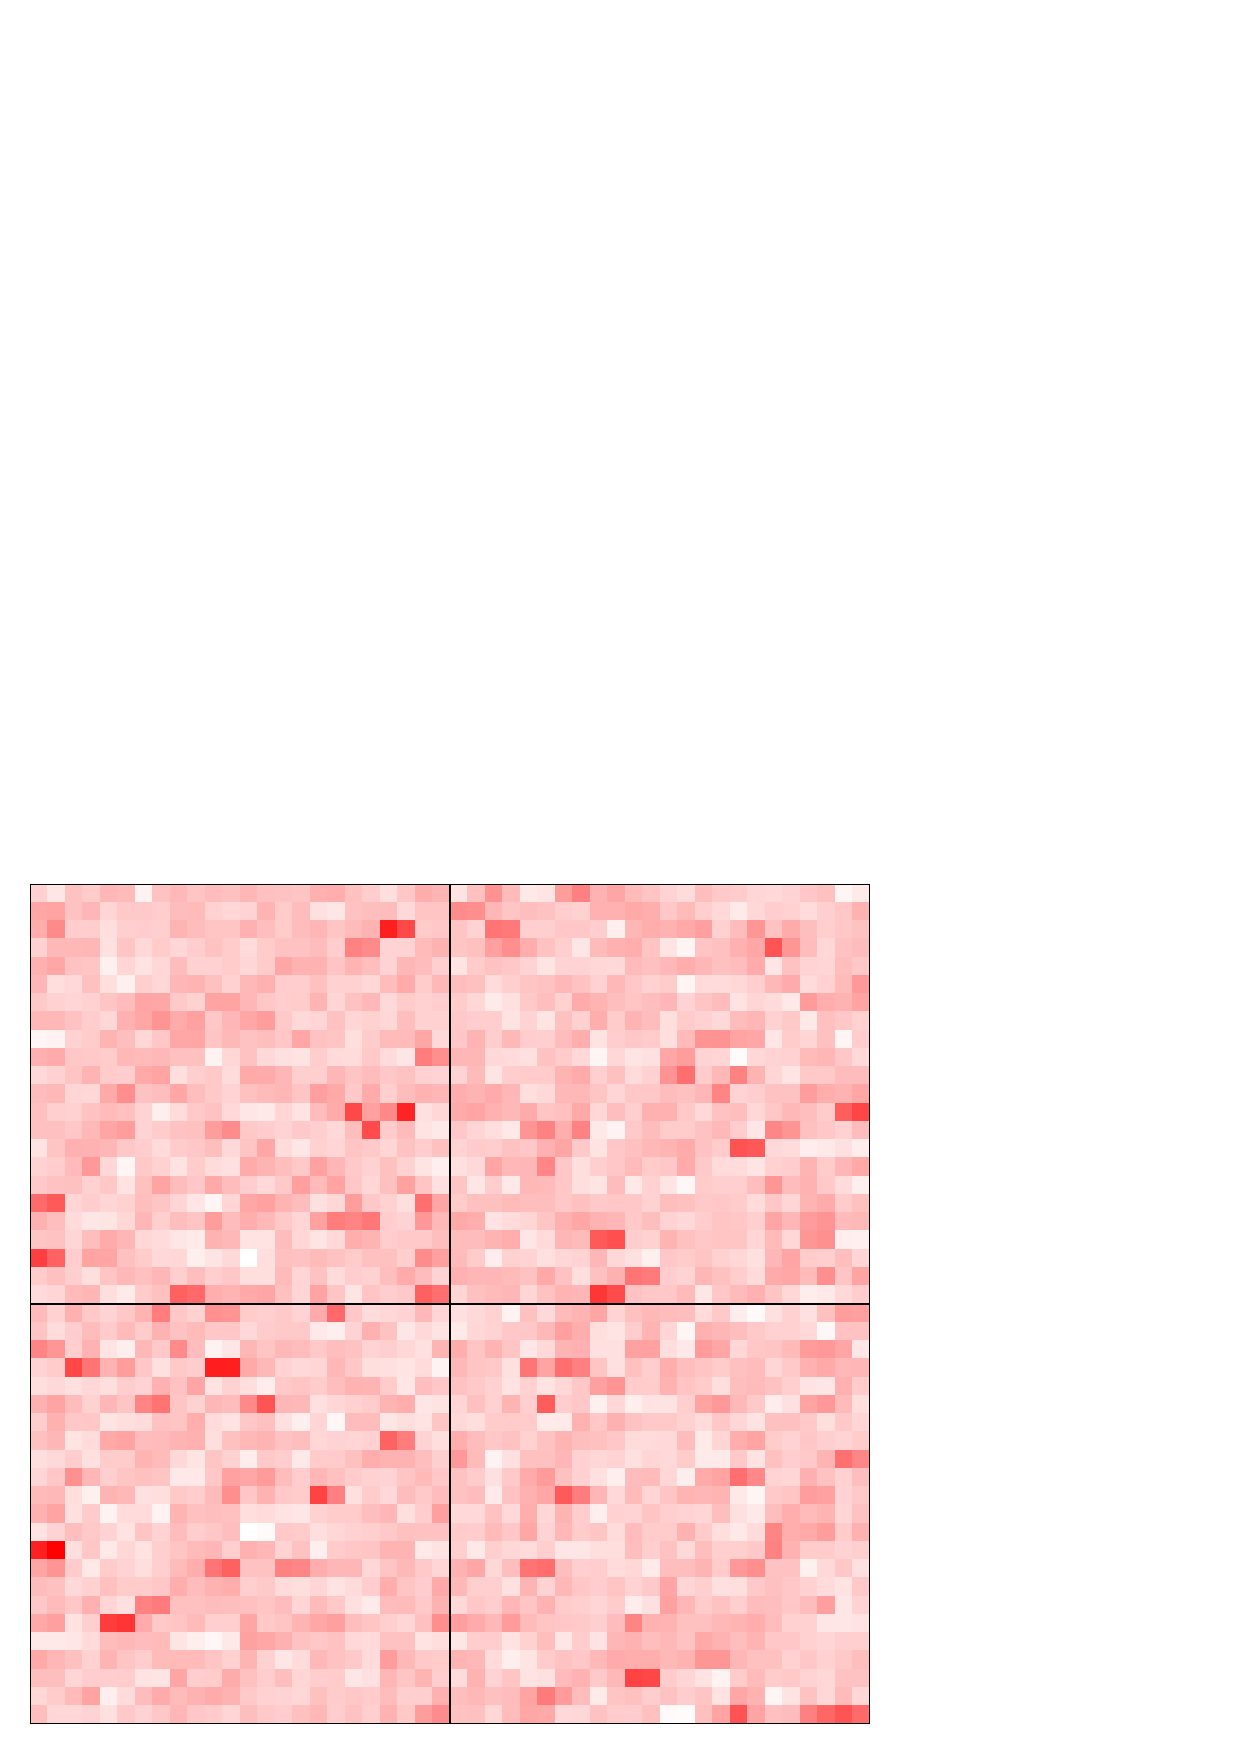
\includegraphics{example-genArise-004}
\caption{Cy3 background preview. \label{fig2}}
\end{center}
\end{figure}
\begin{Scode}
> data(Simon)
> datos <- attr(Simon, "spotData")# Extract spot data
> R <- log(datos$BgCy3, 2)
> imageLimma(z = R, row = 23, column = 24, meta.row = 2, 
  meta.column = 2, low = "white", high = "red")
\end{Scode}

\begin{Soutput}
Output: Cy3 Background value
\end{Soutput}
And this is the plot for Cy5 background.
\begin{figure}[h]
\begin{center}
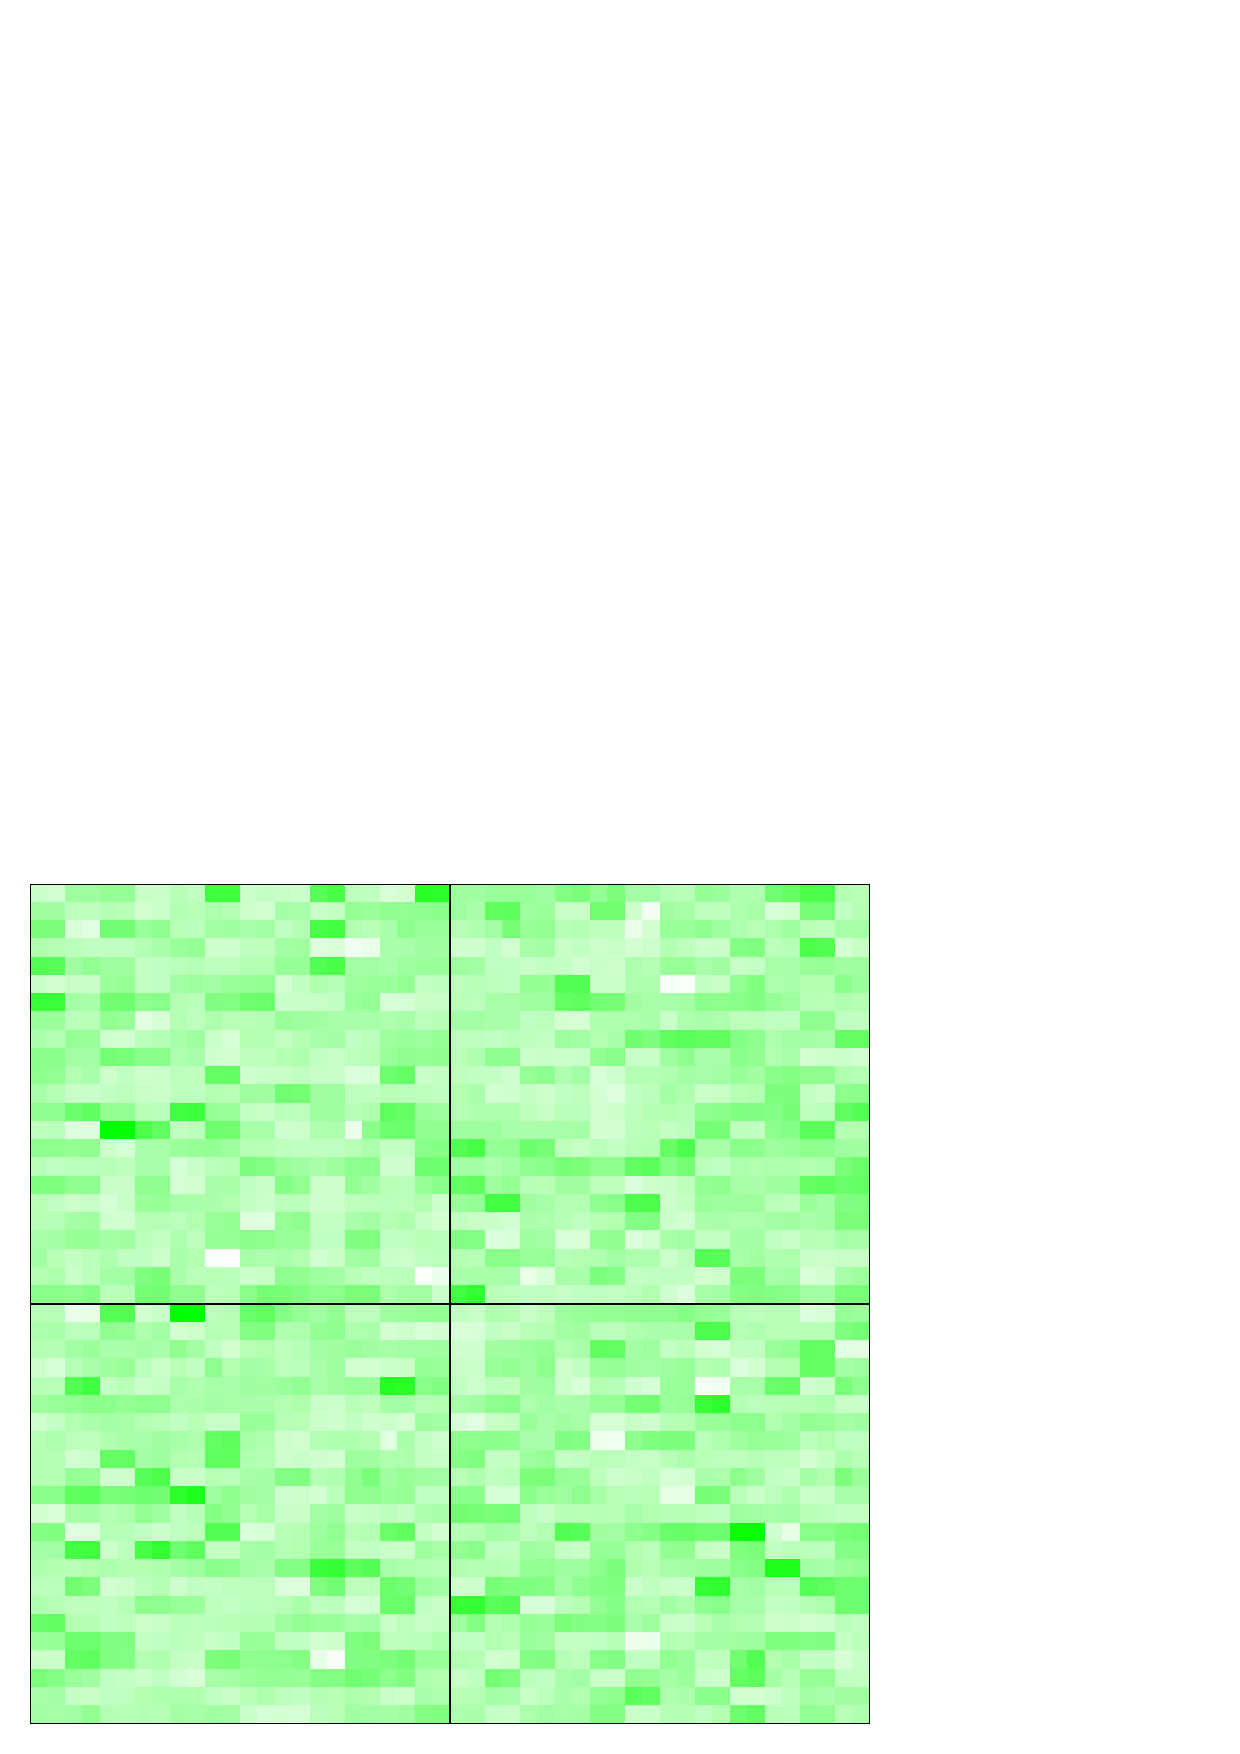
\includegraphics{example-genArise-005}
\caption{Cy5 background preview. \label{fig3}}	
\end{center}
\end{figure}
\begin{Scode}
> data(Simon)
> datos <- attr(Simon, "spotData")# Extract spot data
> G <- log(datos$BgCy5, 2)
> imageLimma(z = G, row = 23, column = 24, meta.row = 2, 
  meta.column = 2, low = "white", high = "green")
\end{Scode}

\begin{Soutput}
Output: Cy5 Background value
\end{Soutput}
With the previous plots, you can see a preview of the raw data (without background correction and normalization).It is important to clarify that these image plot one does not replace the original TIFF image from the microarray experiment.\\

Data analysis requires to be able to plot a spot after apply any operation and genArise provides functions for this purpose. For example, we can plot the values R vs I, M vs A and Cy5 vs Cy3. This functions receive an object of the class Spot.
\begin{figure}[h]
\begin{center}
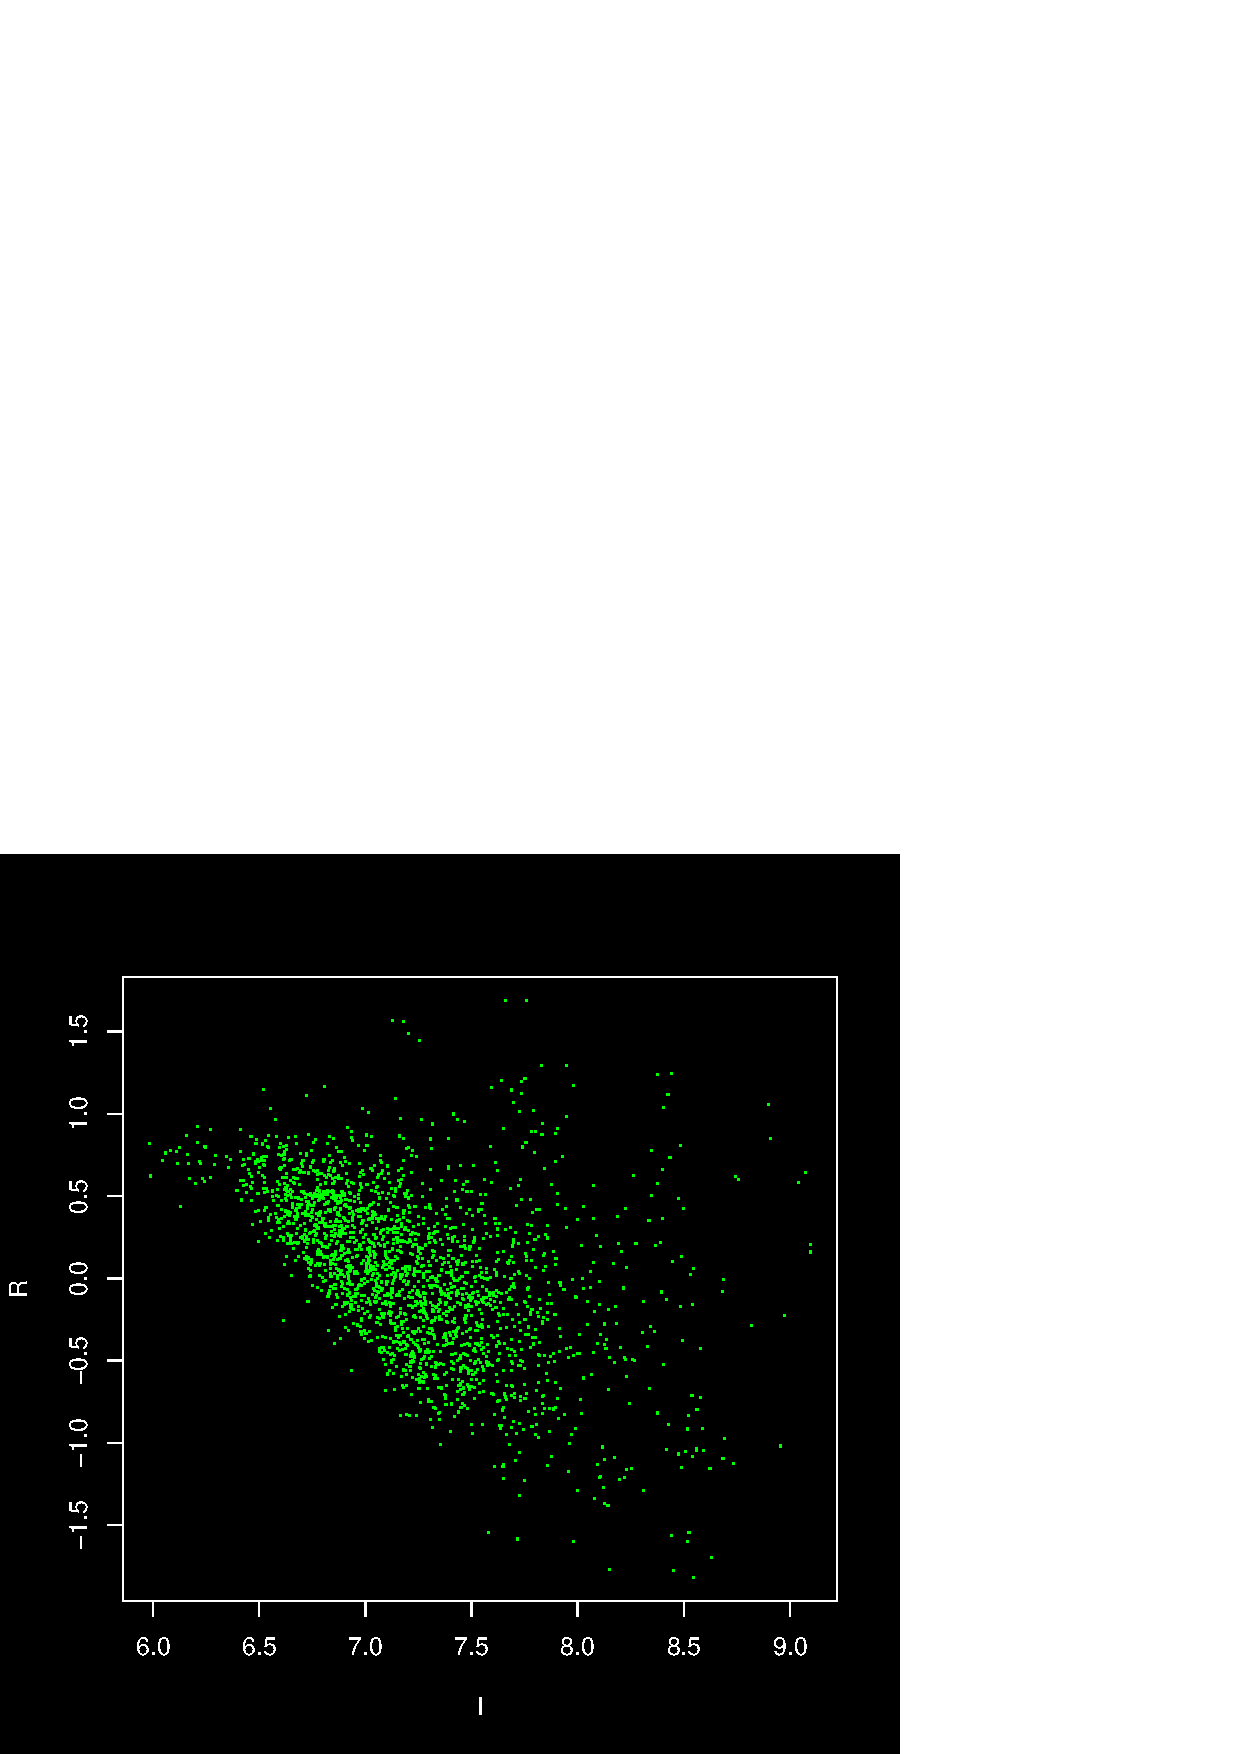
\includegraphics{example-genArise-006}
\caption{R vs I plot. \label{fig4}}	
\end{center}
\end{figure}
\begin{Scode}
> data(Simon)
> ri.plot(Simon)
\end{Scode}
\begin{Soutput}
Output: R vs I plot. See Figure 4.
\end{Soutput}
\begin{figure}[h]
\begin{center}
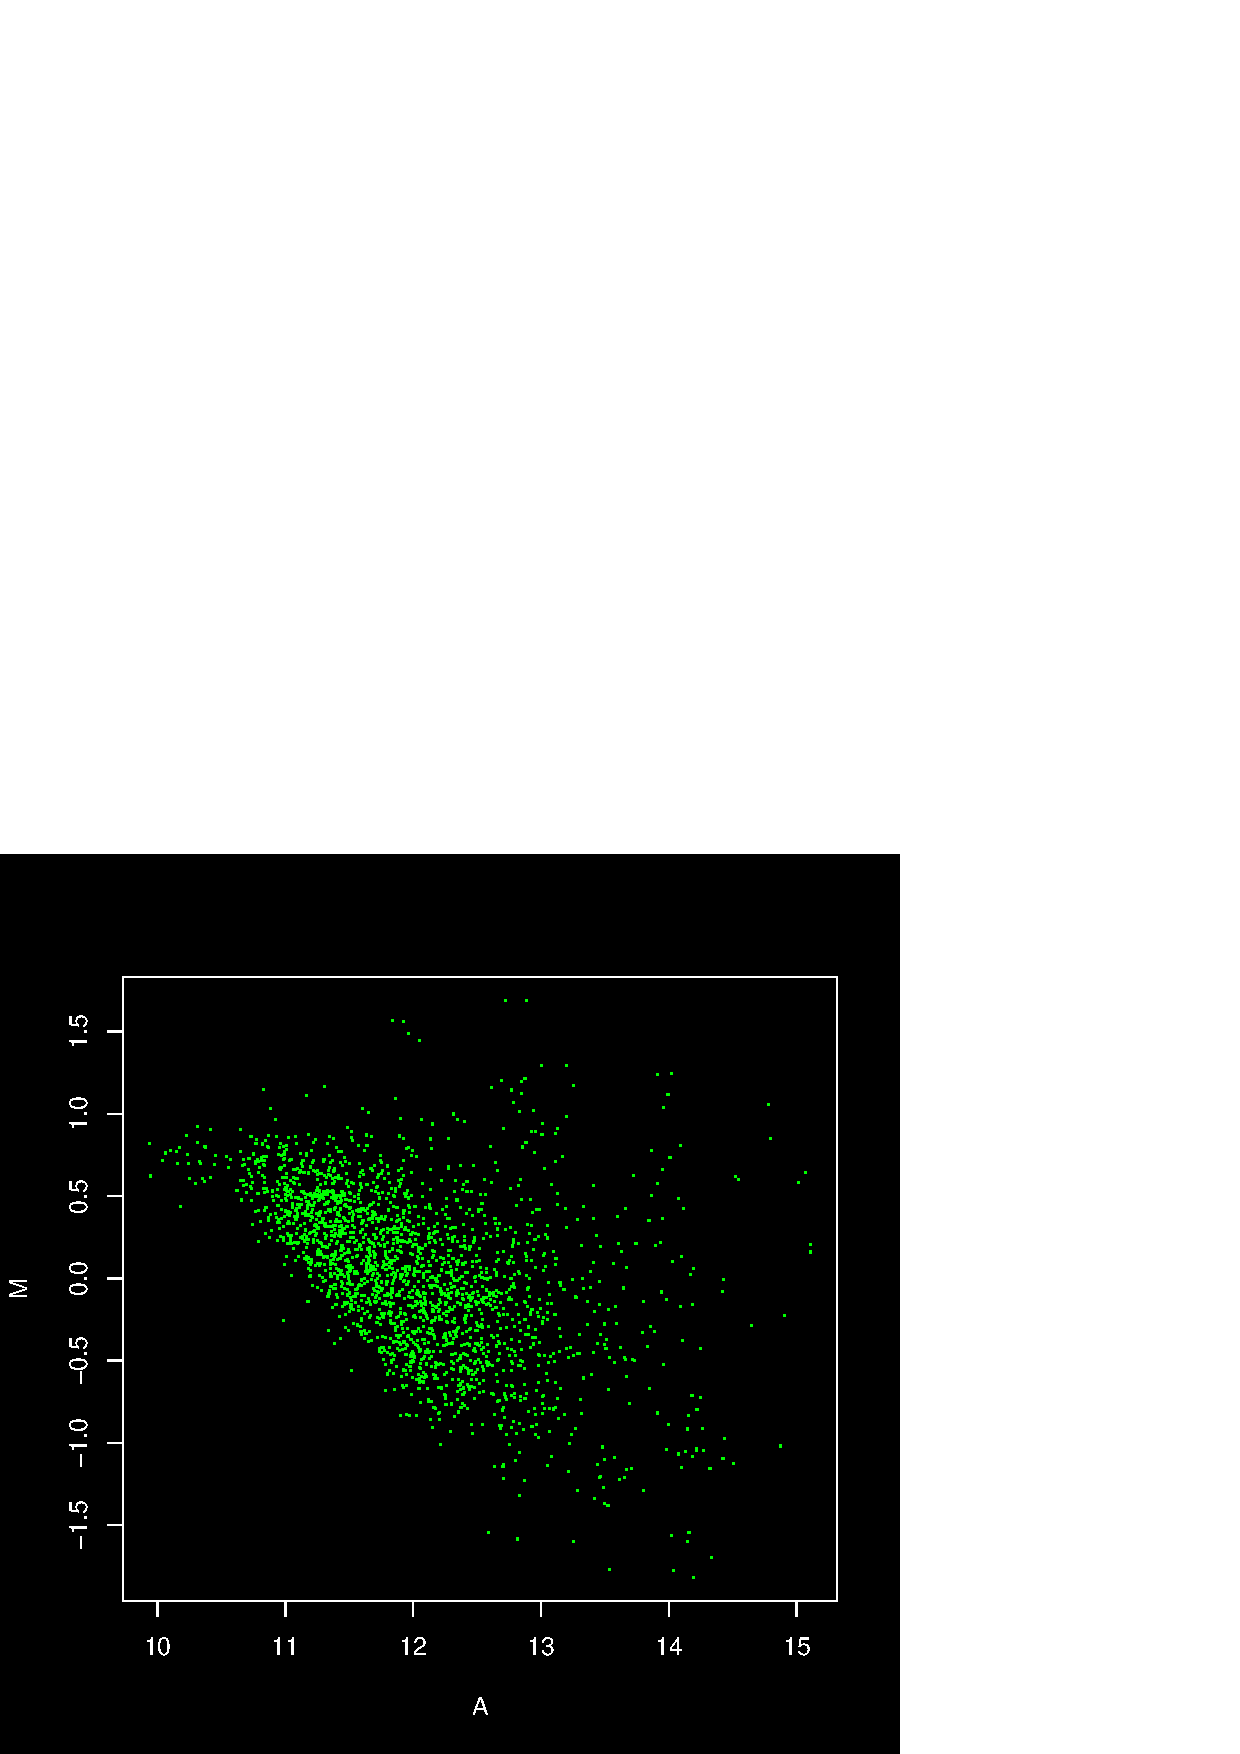
\includegraphics{example-genArise-007}
\caption{M vs A plot. \label{fig5}}
\end{center}
\end{figure}
\begin{Scode}
> data(Simon)
> ma.plot(Simon)
\end{Scode}
\begin{Soutput}
Output: M vs A plot. See Figure 5.
\end{Soutput}
\begin{figure}[h]
\begin{center}
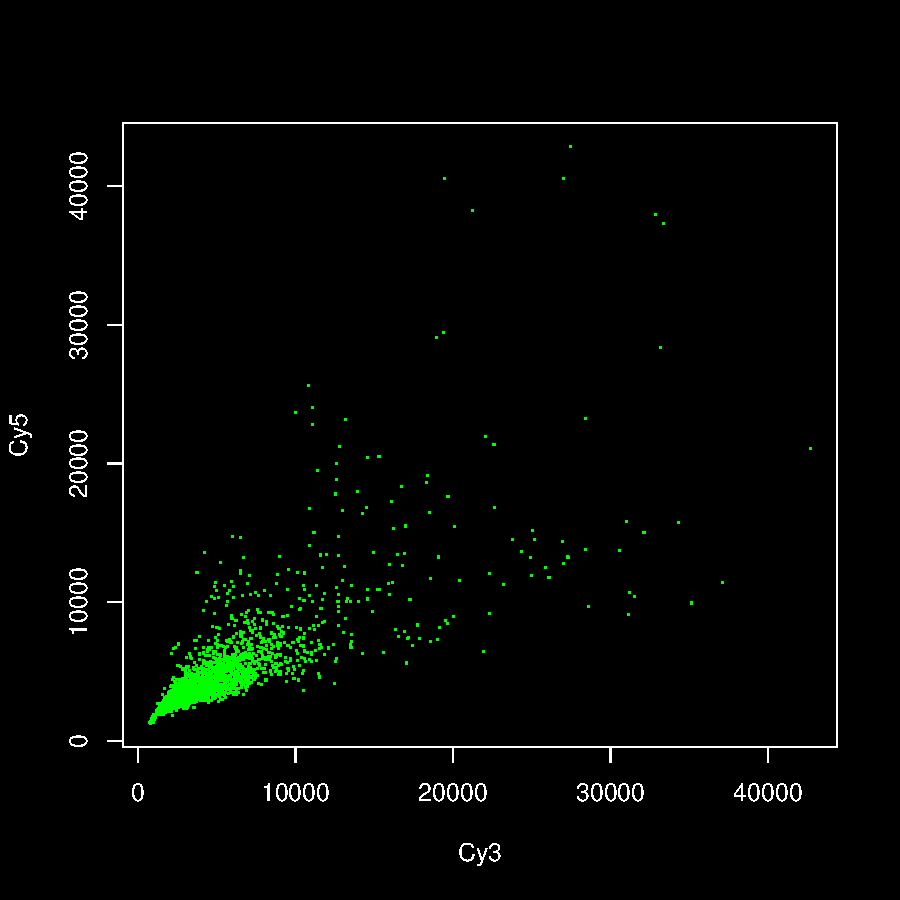
\includegraphics{example-genArise-008}
\caption{Cy3 vs Cy5 plot. \label{fig6}}
\end{center}
\end{figure}
\begin{Scode}
> data(Simon)
> cys.plot(Simon)
\end{Scode}
\begin{Soutput}
Output: plot the Cy3 and Cy5 values. See Figure 6.
\end{Soutput}
At this moment, you can proceed with the data analysis. There are different functions for this purpose. The first of them makes the background correction; that is a subtraction Cy3 - BckgCy3 and Cy5 - BckgCy5 for each spot. See Figure \ref{fig7}. The name of this function is \texttt{bg.correct}.
\begin{figure}[h]
\begin{center}
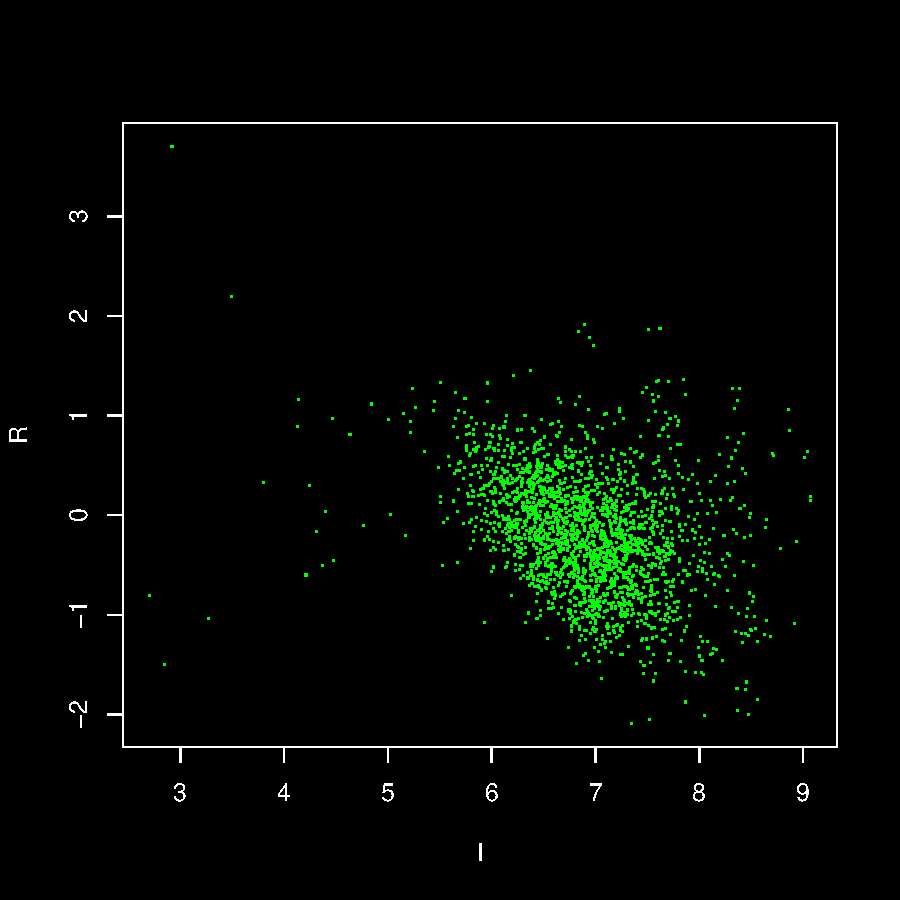
\includegraphics{example-genArise-009}
\caption{R vs I plot of backgroung corrected data. \label{fig7}}
\end{center}
\end{figure}
\begin{Scode}
> data(Simon)
> c.spot <- bg.correct(Simon)
> ri.plot(c.spot)
\end{Scode}

\begin{Soutput}
input: The argument of this function is a spot object
output: A spot object with the corrected background
\end{Soutput}

Data normalization can be done by grids or in a global way, and each method returns different results for the same input data set. We must remark that the grid normalization can just be applied to the complete data set, so you must not eliminate spots in order to avoid errors executing this function.  In the normalization procedure any observation in which the R value is zero will be eliminated.\\

Grid normalization is executed with the function \texttt{grid.norm()} and is mandatory to indicate the dimensions of the subgrid, so, you must indicate the number of rows and columns within each subgrid. See Figure \ref{fig8}.
\begin{figure}[h]
\begin{center}
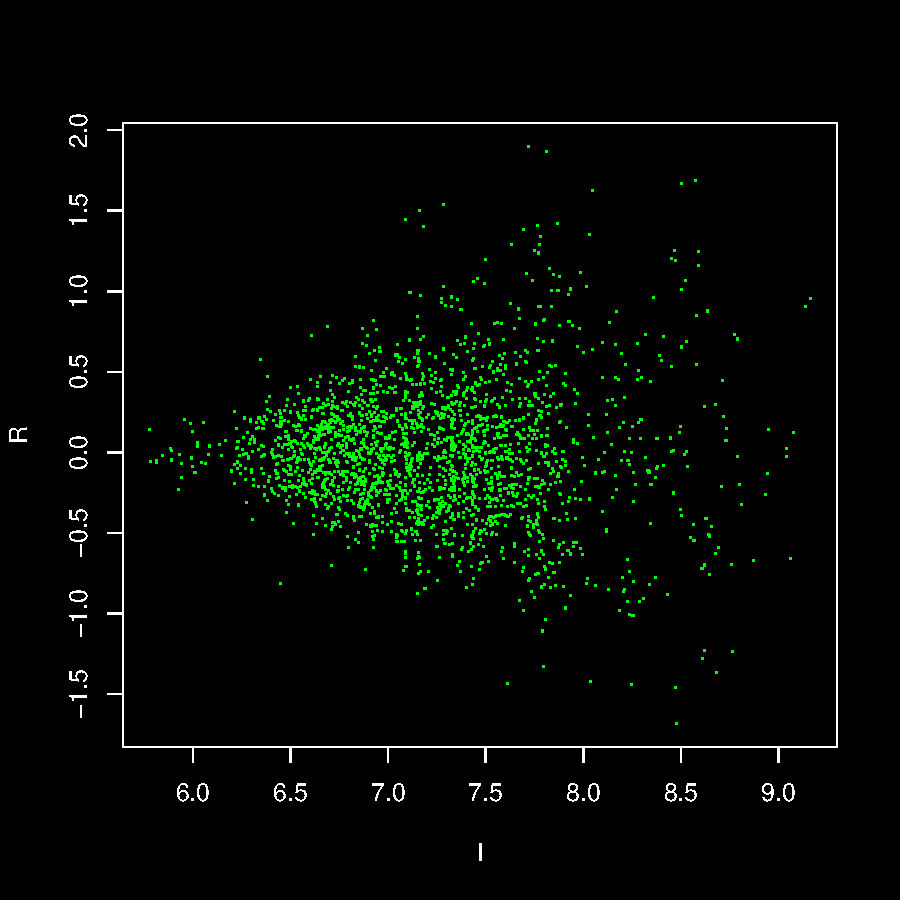
\includegraphics{example-genArise-010}
\caption{R vs I plot of grid normalized data.\label{fig8}}	
\end{center}
\end{figure}
\begin{Scode}
> data(Simon)
> n.spot <- grid.norm(mySpot = Simon, nr = 23, nc = 24)
> ri.plot(n.spot)
\end{Scode}

\begin{Soutput}
input: The argument of this function is a spot object
       and the number of rows (nr) and columns (nc) of each subgrid.
output: A normalized spot object
\end{Soutput}

On the other hand, the global normalization is executed with the function \texttt{global.norm} and it only requires as argument an object of the class Spot. See Figure \ref{fig9}.

\begin{figure}[h]
\begin{center}
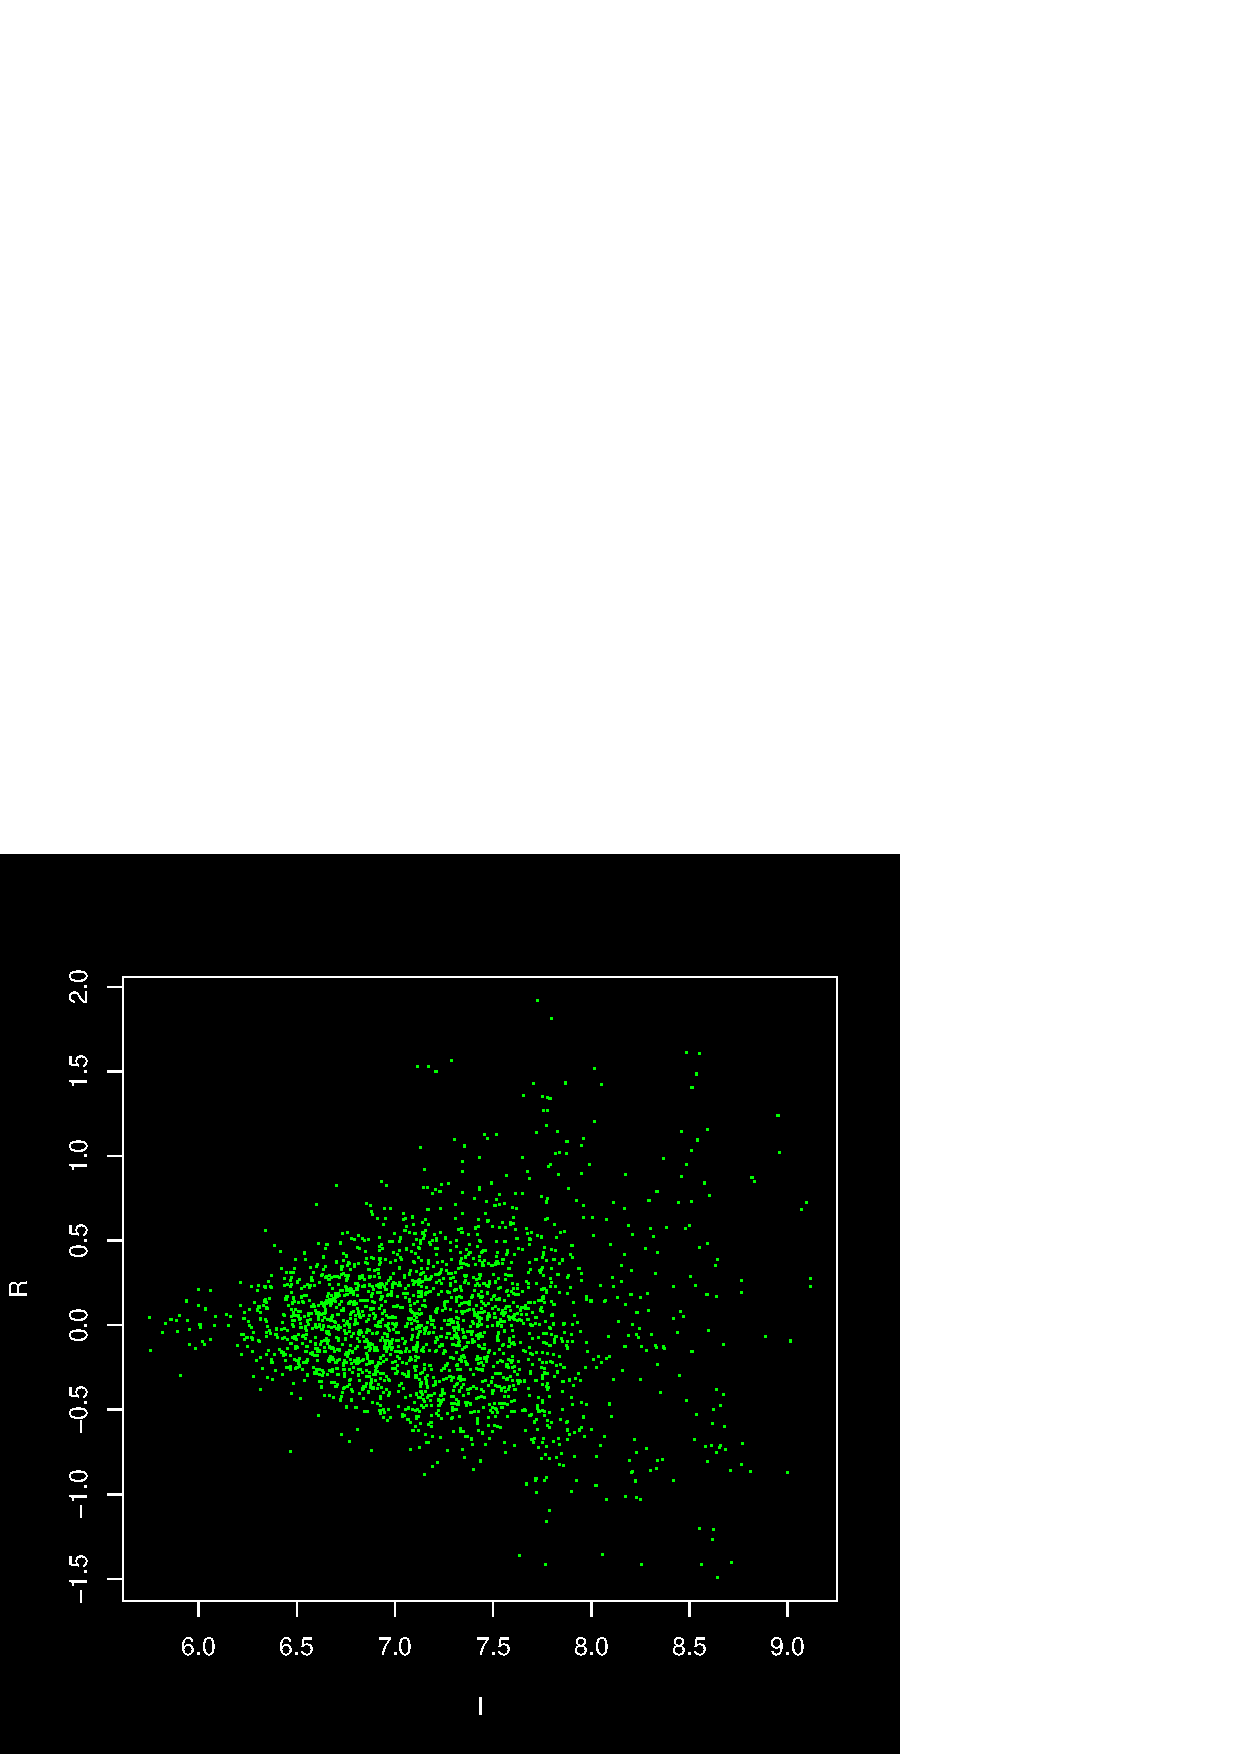
\includegraphics{example-genArise-011}
\caption{R vs I plot of data after global normalization. \label{fig9}}
\end{center}
\end{figure}
\begin{Scode}
> data(Simon)
> n.spot <- global.norm(mySpot = Simon)
> ri.plot(n.spot)
\end{Scode}
\begin{Soutput}
Input: The argument of this function is a spot object
Output: A normalized spot object
\end{Soutput}

As we said previously both functions returns different results and for this reason you must choose the suitable function of normalization to the analysis that we want to do. It for any reason spots are eliminated before normalization procedure (applying operations as filtering or duplicates elimination) the global normalization is the only normalization way.\\

In this example, the number of data in the spot is small and for this reason the obtained values with both normalization functions could seems very similar in the plots, however this is not the same in all the cases.\\

Data filtering is an important step too in the data analysis. genArise implements the intensity-based filtering algorithm described by John Quackenbush\footnote[2]{ John Quackenbush \textquotedblleft Microarray data normalization and transformation\textquotedblright. Nature Genetics. Vol.32 supplement pp 496-501 (2002)}. After this filtering you keep only array elements with intensities that are statistically significantly different from background. See Figure \ref{fig10}.\\

\begin{figure}[h]
\begin{center}
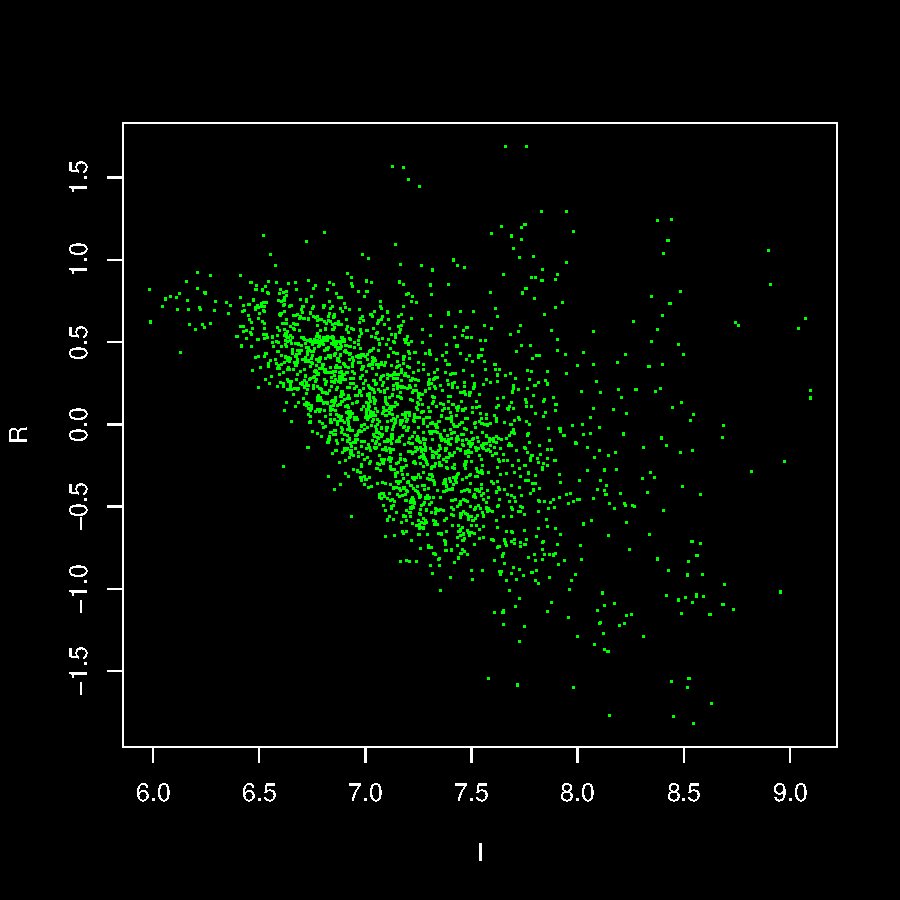
\includegraphics{example-genArise-012}
\caption{Filtered data, R vs I plot. \label{fig10}}	
\end{center}
\end{figure}

\begin{Scode}
> data(Simon)
> f.spot <- filter.spot(mySpot = Simon)
> ri.plot(f.spot)
\end{Scode}

\begin{Soutput}
Input: The argument of this function is a spot object.
Output: A spot filtering spot object
\end{Soutput}

Another step is the replicates filtering, and in this step, a lot of observations are eliminated. We can not just conserve the half of points, but also this function eliminates those points where the diference between the R value of the duplicated observations is bigger than 20\% of one of them. See Figure \ref{fig11}.\\
\begin{figure}[h]
\begin{center}
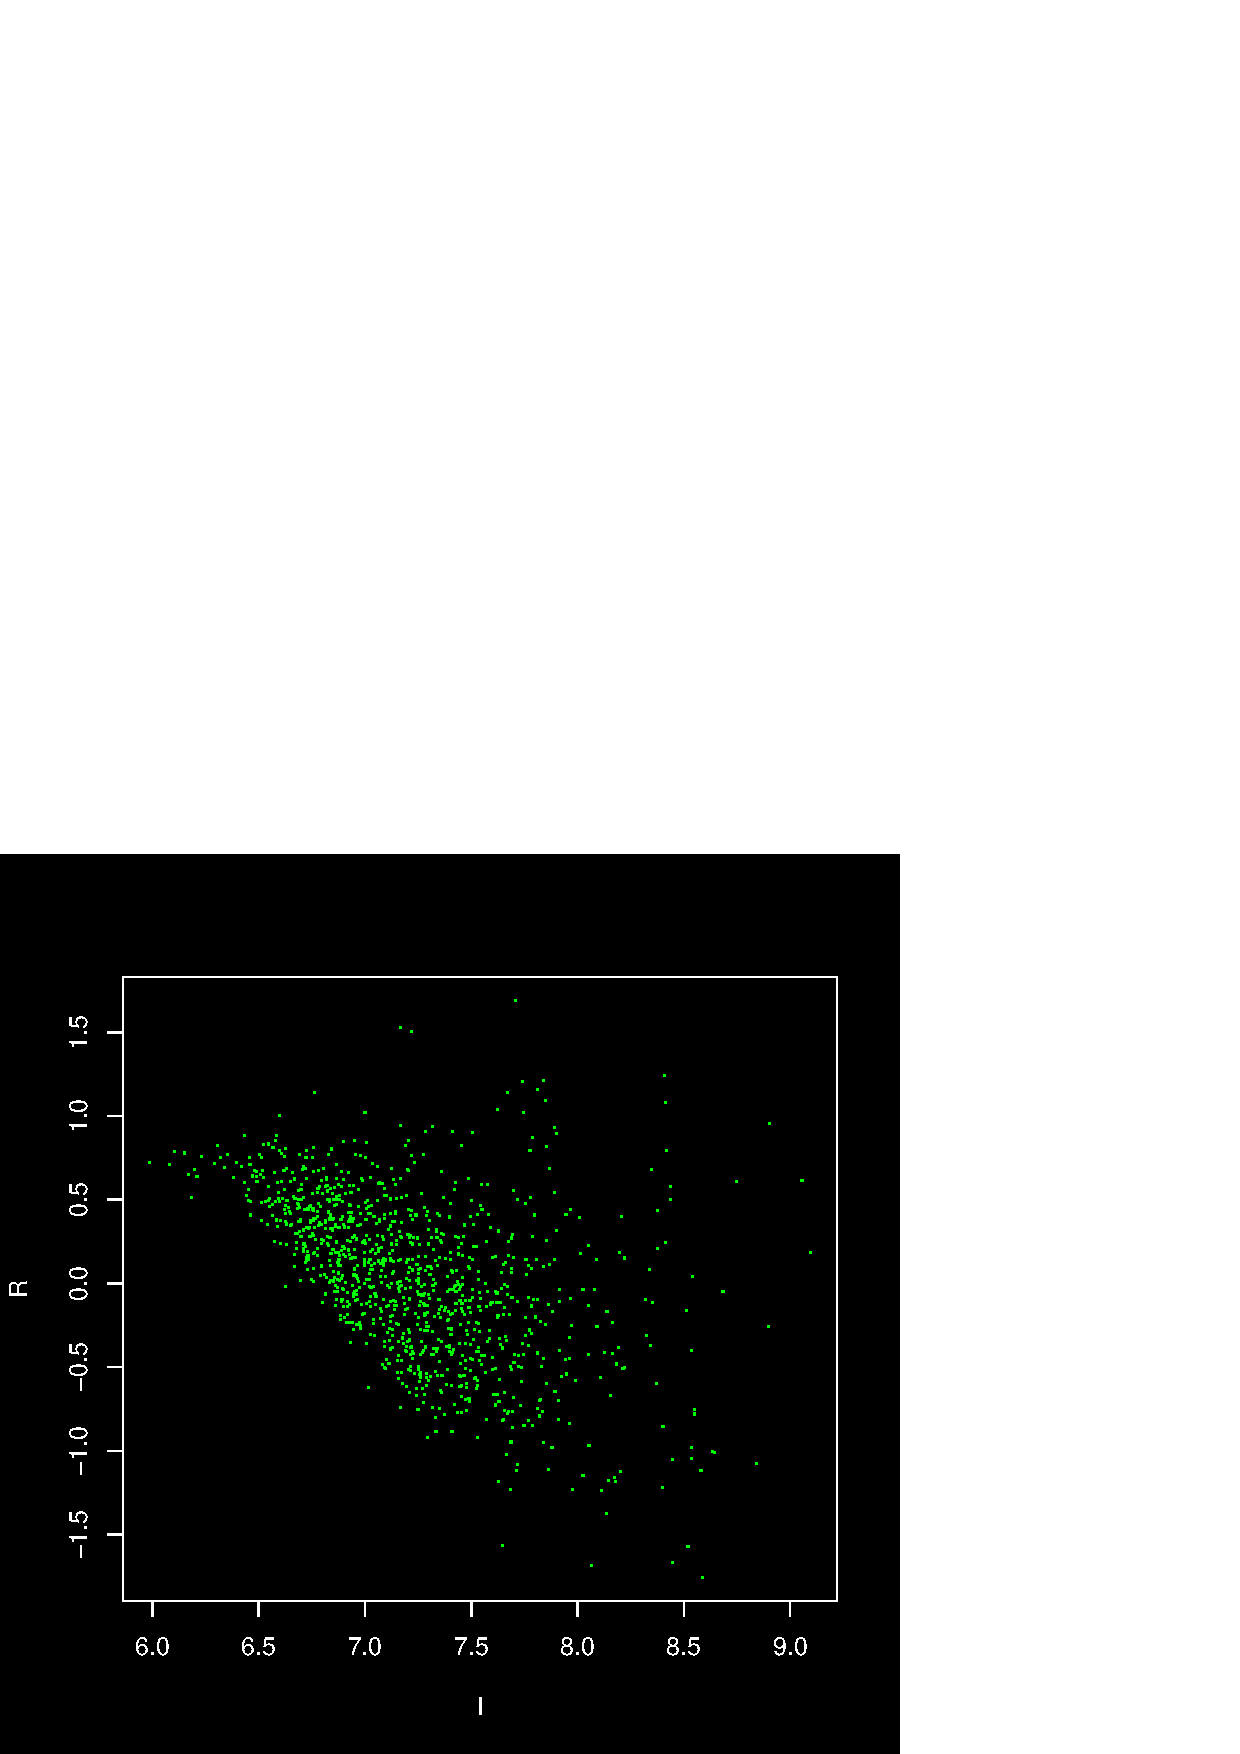
\includegraphics{example-genArise-013}
\caption{R vs I plot of data after apply \texttt{spotUnique} function. \label{fig11}}
\end{center}
\end{figure}
\begin{Scode}
> data(Simon)
> u.spot <- spotUnique(mySpot = Simon)
> ri.plot(u.spot)
\end{Scode}

\begin{Soutput}
Input: The argument of this function is a spot object.
Output: A spot object without duplicates observations
\end{Soutput}

However, genArise offers other functions for the elimination of duplicates different from the previous one. We talk about the function \texttt{alter.unique}. This function takes the R value of each one of the duplicated observations but just keep that observation with the extremest R value. So, if both of them are positives this function keeps the greater one, if both of them are negatives it keep the lower one and if there is one positive and one negative both observations are eliminated. It is clear that with this function a greater number of observations is conserved compared to those that are obtained with \texttt{spotUnique} function. By this way you will probably have at the final of the analysis a greater number of observations in the upper-expressed and lower-expressed because you keep the extreme values. See Figure \ref{fig12}.\\
\begin{figure}[h]
\begin{center}
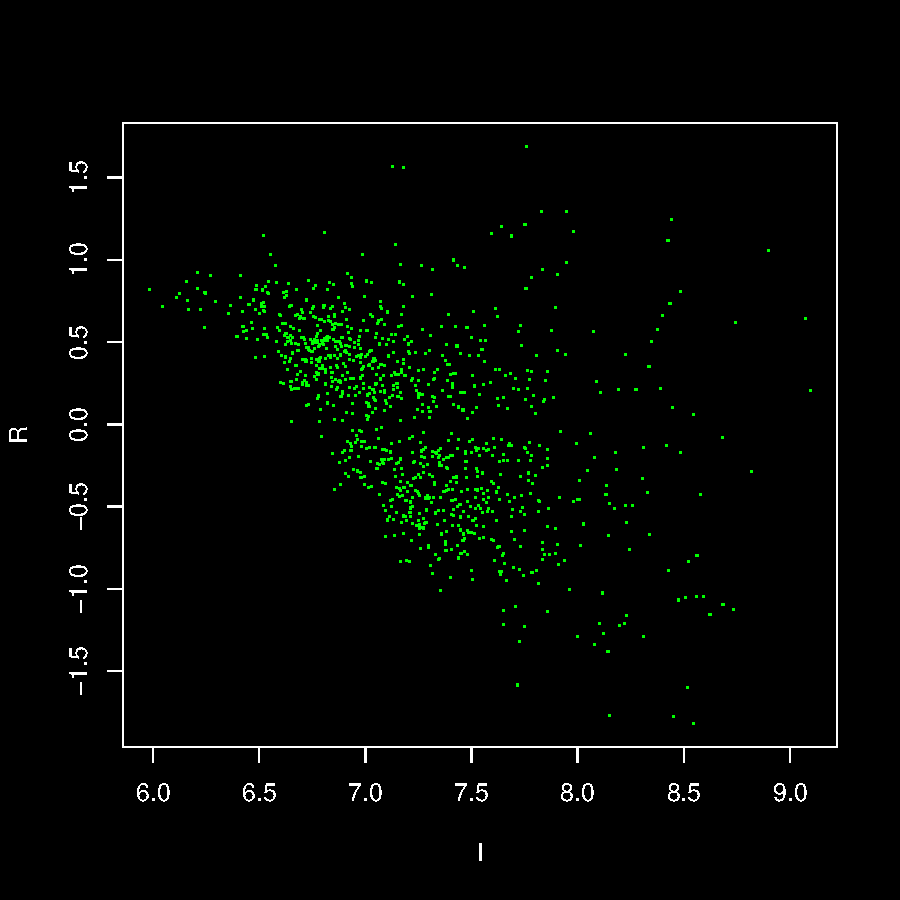
\includegraphics{example-genArise-014}
\caption{R vs I plot of data after apply \texttt{alter.unique} function.\label{fig12}}
\end{center}
\end{figure}
\begin{Scode}
> data(Simon)
> u.spot <- alter.unique(mySpot = Simon)
> ri.plot(u.spot)
\end{Scode}

\begin{Soutput}
input: The argument of this function is a spot object.
output: A spot object without duplicates observations
\end{Soutput}

The other fuction just get the mean of the duplicates and perform the filtering. The name of this function is \texttt{meanUnique}. See Figure \ref{fig13}.

\begin{figure}[h]
\begin{center}
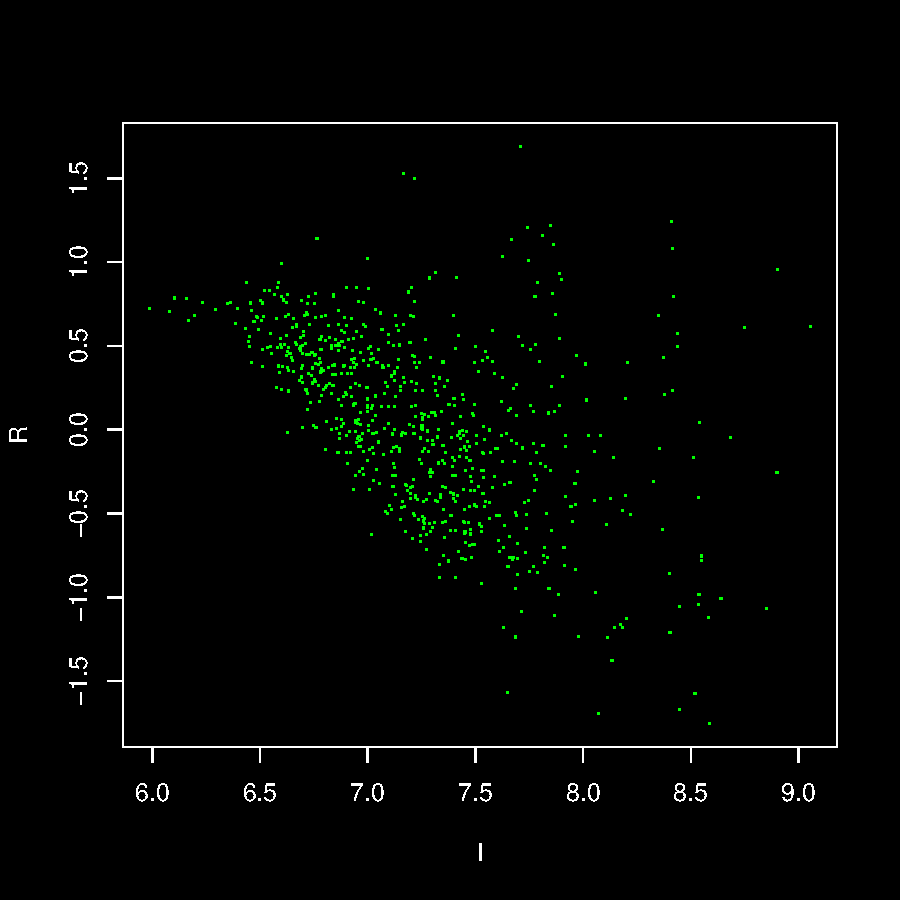
\includegraphics{example-genArise-015}
\caption{R vs I plot of data after apply \texttt{meanUnique} function.\label{fig13}}
\end{center}
\end{figure}
\begin{Scode}
> data(Simon)
> u.spot <- meanUnique(mySpot = Simon)
> ri.plot(u.spot)
\end{Scode}

\begin{Soutput}
input: The argument of this function is a spot object
output: A spot object without duplicates observations
\end{Soutput}

The approach we use involves calculating the mean and standard deviation of the distribution of $log_2$(ratio) values and defining a global fold-change difference and confidence; for this we use a Z-score for the data set. In an R-I plot, that would be represented as parallel horizontal lines; genes outside of those lines would be the differentially expressed\footnotemark[2]. See Figure \ref{fig14}.\\

As a matter of fact genArise offers two options for this analysis. You just need to specify in the type argument on the \texttt{Zscore} function if you want a R-I or a M-A analysis. This function receive as argument an object of the class Spot and returns an object of other class called DataSet that includes as one of their values the Z-score for the data set.\\

This is the example for \texttt{Zscore} using  R-I values.

\begin{Scode}
> data(Simon)
> s.spot <- Zscore(Simon, type="ri")
\end{Scode}

\begin{Soutput}
Input: The argument of this function is a spot object
Output: An object of the class DataSet
\end{Soutput}

And this is the example for \texttt{Zscore} using \texttt{M-A} values

\begin{Scode}
> data(Simon)
> s.spot <- Zscore(Simon, type="ma")
\end{Scode}

\begin{Soutput}
Input: The argument of this function is a spot object
Output: An object of the class DataSet
\end{Soutput}

Since the objects of the class \texttt{DataSet} are different from the objects of the class Spot we need a function to plot them. For this purpose exists a function called \texttt{Zscore.plot}. So, in a R-I plot, array elements are color-coded depending on wether they are less than 1 standard deviation from the mean (blue), between 1 and 1.5 standard deviations (green), between 1.5 and 2 standard deviations (red), or more than 2 standard deviations from the mean (orange).
\begin{figure}[h]
\begin{center}
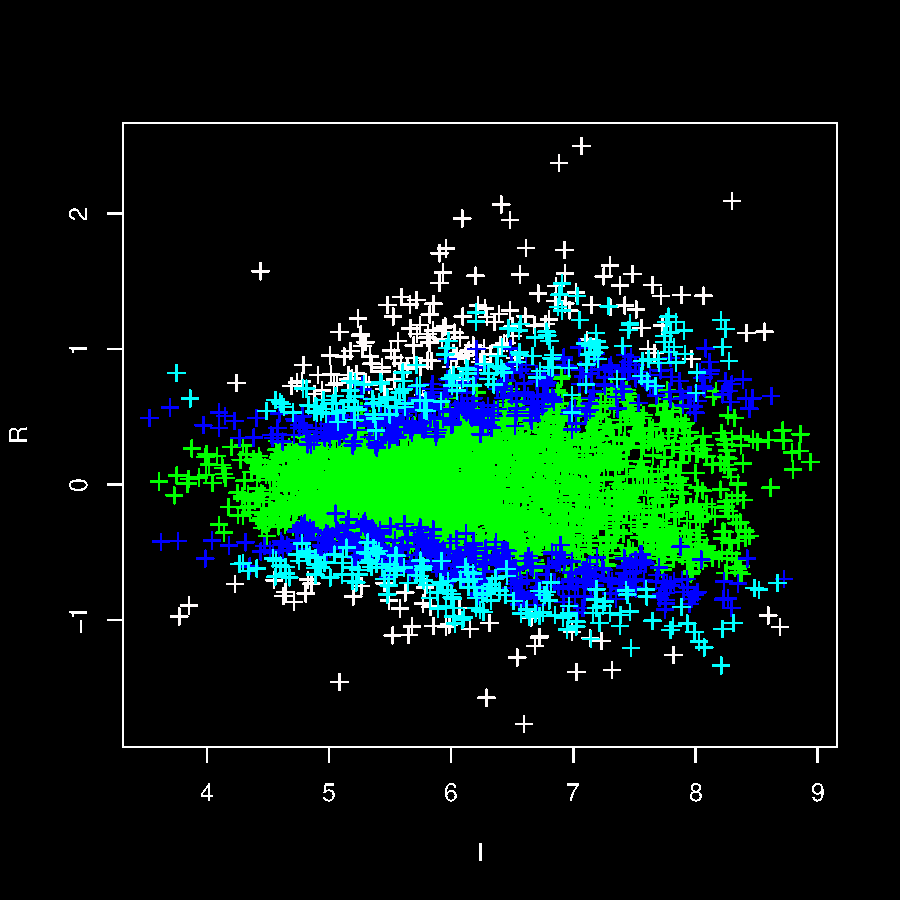
\includegraphics{example-genArise-016}
\caption{Data after Z-score Analysis. \label{fig14}}
\end{center}
\end{figure}
\begin{Scode}
> data(WT.dataset)
> Zscore.plot(WT.dataset)
\end{Scode}

\begin{Soutput}
Input: An object of the class DataSet
Output: Plot for identify differential expression
\end{Soutput}

After we finished our slice analysis we get a up-regulated and down-regulated set. This will be the set of study genes for genMerge. Given this set, genMerge retrieves functional genomic data for each gene and provides statistical rank scores for over-representation of particular functions in the dataset. The \texttt{genMerge} function is completly based on GeneMerge from Cristian I. Castillo-Davis and Daniel L. Hartl \footnote[3]{Cristian I. Castillo-Davis, Department of Statistics, Harvard University \url{http://www.oeb.harvard.edu/hartl/lab/publications/GeneMerge}
}.\\

Given a set of genes (for example the upper-expressed), genMerge write in files the data of an statistic analysis of the upper/representation of functions or particular categories on the set of data upper-expressed.\\

You must take care in the format of the input file, the file must not have a header row. This function requires four data files and the file name where will be save the obtained information. The main file that the function needs are:\\\\

\textbf{Association file}. This file contains two columns splited by tab characters. The first column corresponds to the gene identifier in the microarray and the second one corresponds to a list of associated ids for the geneontology database to this gen (GO). Each GO in this list is separted by ";" and is necessary to consult a database to locate the associated GOs to each gen (see http://www.geneontology.org)
\begin{Scode}
Example:

YAL001C GO:0003709;
YAL002W GO:0005554;
YAL003W GO:0003746;
YAL005C GO:0003754;GO:0003773;GO:0004002;
YAL007C GO:0005554;
\end{Scode}

\textbf{Description file}. This file also contains two columns splited by tab characters, the first one corresponds to the name of some GOs and the second one corresponds to the description associated to each GO in the database.
\begin{Scode}
Example:

GO:0000005      ribosomal chaperone activity
GO:0000006      high affinity zinc uptake transporter activity
GO:0000007      low-affinity zinc ion transporter activity
GO:0000008      thioredoxin
GO:0000009      alpha-1,6-mannosyltransferase activity
GO:0000010      trans-hexaprenyltranstransferase activity
GO:0000014      single-stranded DNA specific endodeoxyribonuclease activity
GO:0000016      lactase activity
\end{Scode}

\textbf{All genes (population.genes)}. This file should only contain one column, the spot identifiers or those of the input file not analyzed yet are the column information, each identifier is a row file. 
\begin{Scode}
YAL001C
YAL002W
YAL003W
YAL004W
YAL005C
YAL007C
YAL008W
YAL009W
YAL010C
YAL011W
\end{Scode}

\textbf{The genes to study}. Like the preceding described file, this file only contains one column and each row corresponds to the name of one of the genes in the set that will be studied (upper-expressed or lower-expressed). The function sintax is the next one:

\begin{Scode}
> # Let's suppose that original spot is o.spot
> # To write the population file you can use write.table
> ids <- attr(o.spot, "spotData")$Ids
> ids <- unique(ids)
> write.table(ids, "population.genes")
\end{Scode}

\begin{Soutput}
Input: An object of class Slice
Output: Plot upper-expressed and lower-expressed
\end{Soutput}

In the same way, with the \texttt{write.table} function you can write the identifiers of the genes set that will be studied. Suppose there exist a slice Spot we call s.spot wich have the results after slice analysis, if you wish that your set of study have the upper-expressed identifiers and the lower-expressed identifiers to write the corresponding file, you must follow the next code.

\begin{Scode}
> # To write the study genes file
> study.ids <- c(s.spot$Id.up, s.spot$Id.down)
> study.ids <- unique(study.ids) 
> write.table(study.ids, "study.genes")
\end{Scode}

If you only want to preserve the identifier of some set, say upper-expressed or lower-expressed type the next lines:

\begin{Scode}
> # Only write upper-expressed
> study.ids <- s.spot$Id.up # to write lower-expressed use s.spot$Id.down
> study.ids <- unique(study.ids)
> write.table(study.ids, "study.genes")
\end{Scode}

The other files should be constructed consulting a database or could be downloaded from the internet, this files should contain the format described above, so that the genMerge function operates correctly. The sintax of this is:   

\begin{Scode}
> genMerge(gene.association, description, population.genes,
  study.genes, output.file = "GeneMerge.txt"){
\end{Scode}

The results will be in the corresponding file, in the above example \texttt{GeneMerge.txt}.

\section{The genArise GUI}

For making the analysis easier, genArise joins all functions in a graphic interface, to call this function we type the next line:

\begin{Scode}
> genArise()
\end{Scode}

Now the next menu-bar is displayed.
\begin{figure}[h]
\begin{center}

\includegraphics[scale= 0.3]{./images/mainmenu.pdf}\\
\caption{genArise Menu-bar. \label{fig15}}
\end{center}
\end{figure}

Once in this menu you should create a New Project following the sequence  \textbf{File $\rightarrow$ Project $\rightarrow$ New Project}.\\
The last step displays a window where you should indicate the file' s location containing the data to analyze, indicating whether the file is a foreing experiment or belong to one made in the Cellular Physiology Institute UNAM. 
\begin{figure}[h]
\begin{center}
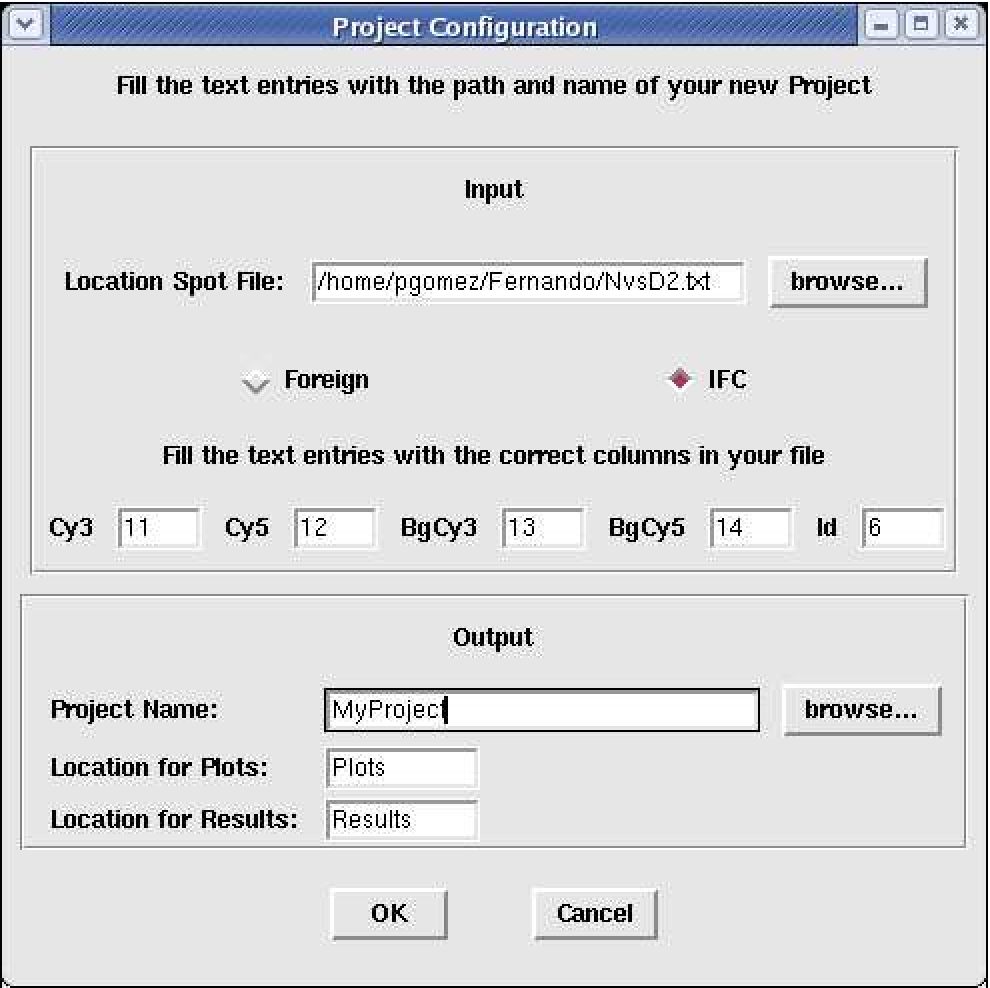
\includegraphics[scale= 0.3]{./images/projectmenufilled.pdf}\\
\caption{Project Configuration Window. \label{fig16}}
\end{center}
\end{figure}

In the lower textfields you should indicate the name of the new project, including the complete path (location where you want to save the project containing the results and graphics obtained during the analysis).\\\\
 For example:\\
 \\
The Figure \ref{fig16} shows an analysis that will be made on the file Rat\_5k\_014.csv containig a microarray made in the Cellular Physiology Institute' s Microarray Unit. We call the project \textquotedblleft ProjectRat \textquotedblright. The default name for the graphics directory is Plot and for the data files is Results. If we wish to modify this names we just change the names that appear in the options \textbf{Location for Plots } and \textbf{Location for Results}, respectively.\\

Then, the window containing a preliminary view of the main grid is displayed as an image plot in a green to red scale representing the $log_2$ intensity ratio for each spot on the array. See Figure \ref{fig17}. It is important to clarify that these image plot one does not replace the original TIFF image from the microarray experiment.

\begin{figure}[h]
\begin{center}
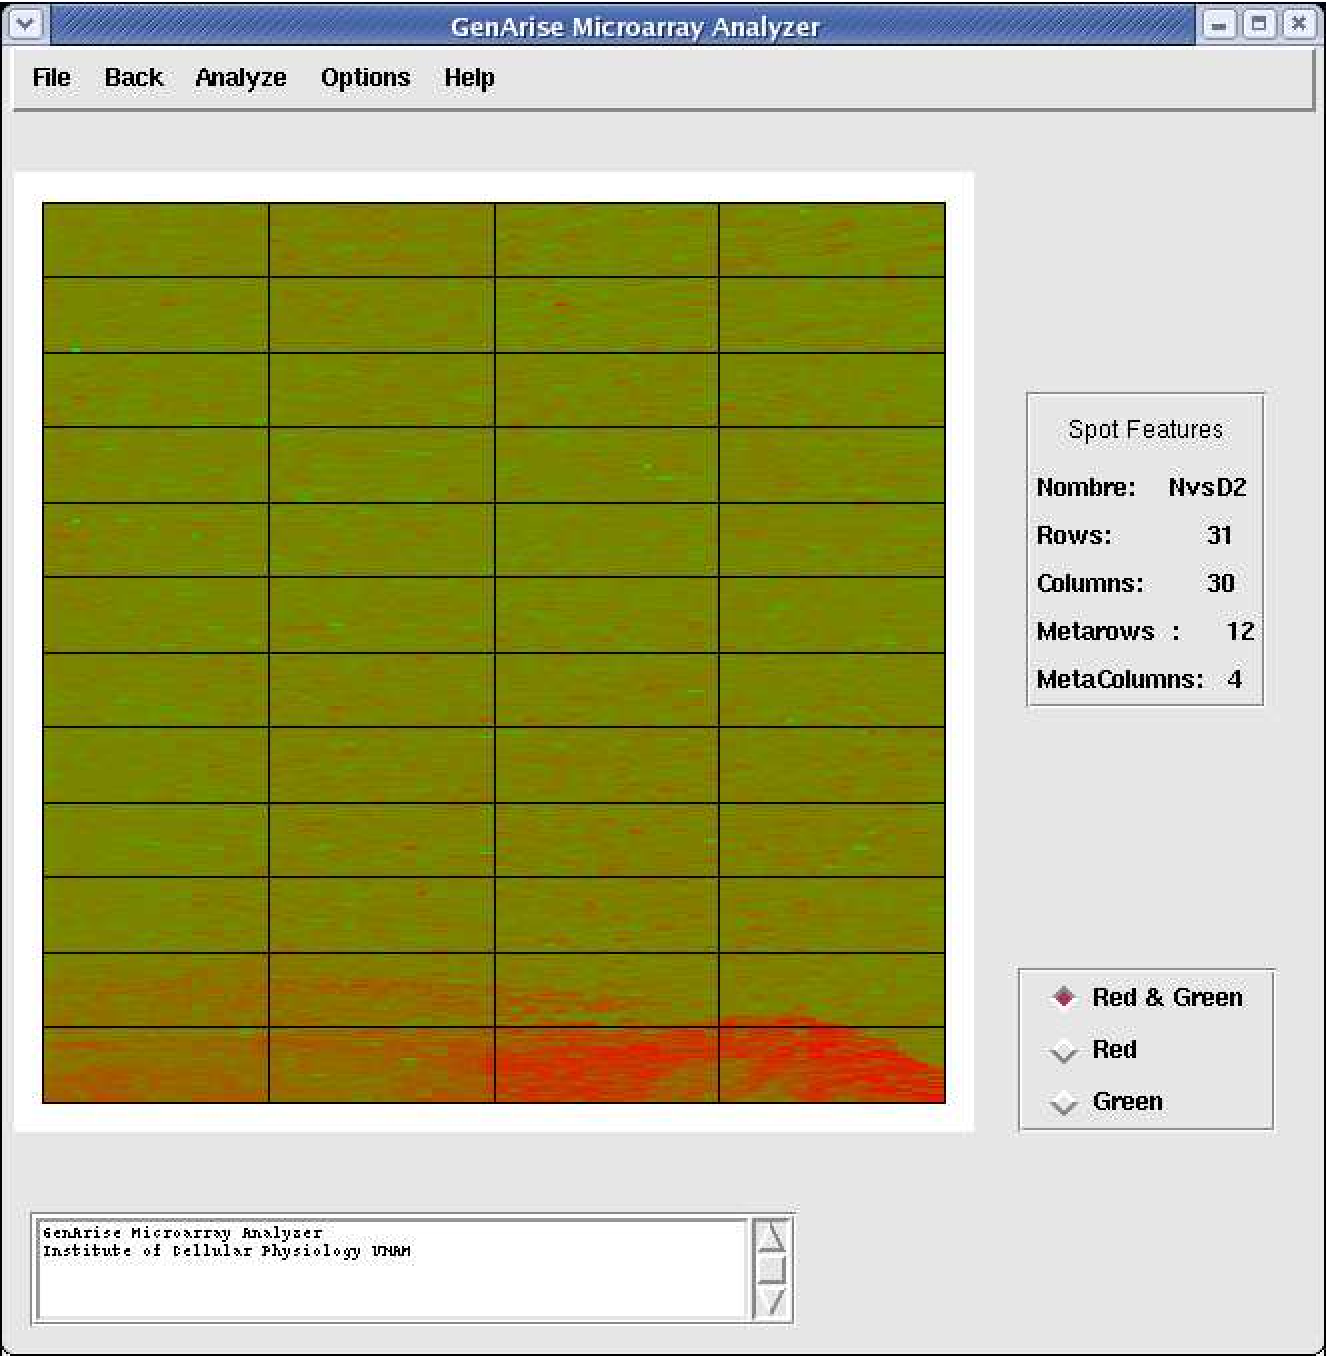
\includegraphics[scale= 0.3]{./images/principal.pdf}\\
\caption{Window with image plot in a green to red scale. \label{fig17}}
\end{center}
\end{figure}
You also can see the green and red levels in a separated form just by selecting the corresponding option in the lower right part of the window. See Figure \ref{fig18} and \ref{fig19}.
\begin{figure}[h]
\begin{center}
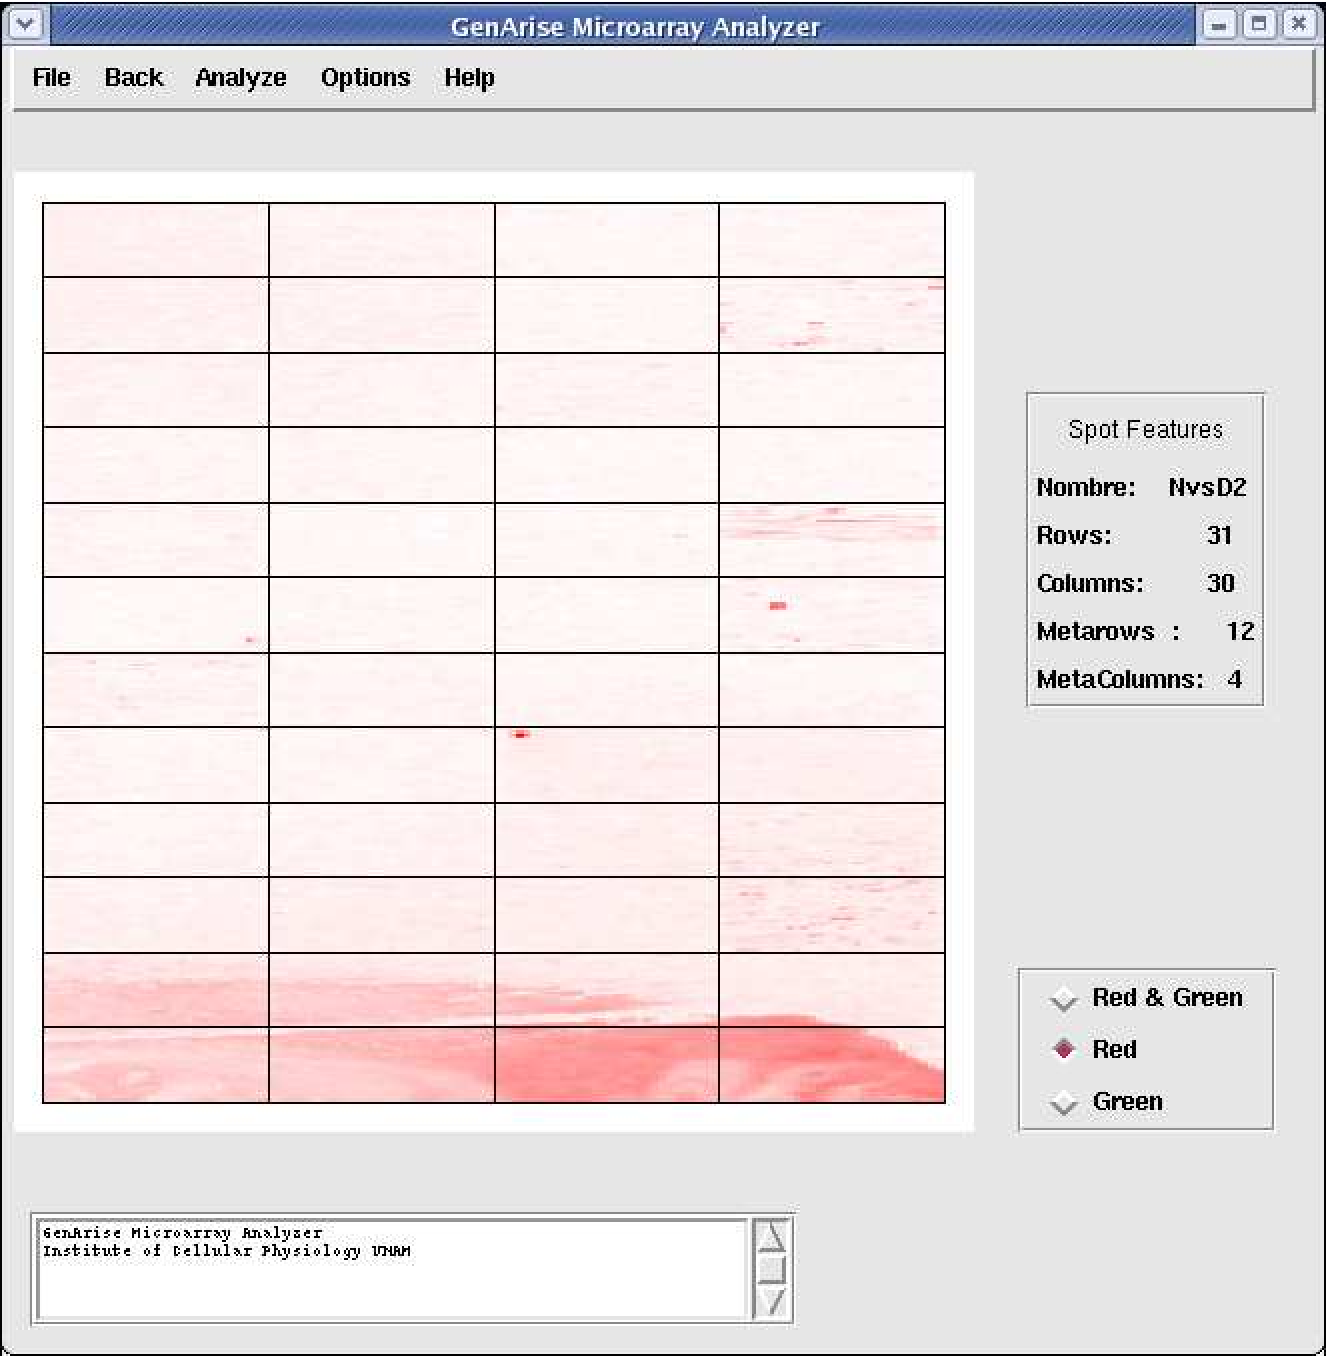
\includegraphics[height=3.in,width=3.15in]{./images/principalRed.pdf}\\
\caption{Window with image plot for Cy3 Background value. \label{fig18}}
\end{center}
\end{figure}
\textbf{\\\\}
\begin{figure}[h]
\begin{center}
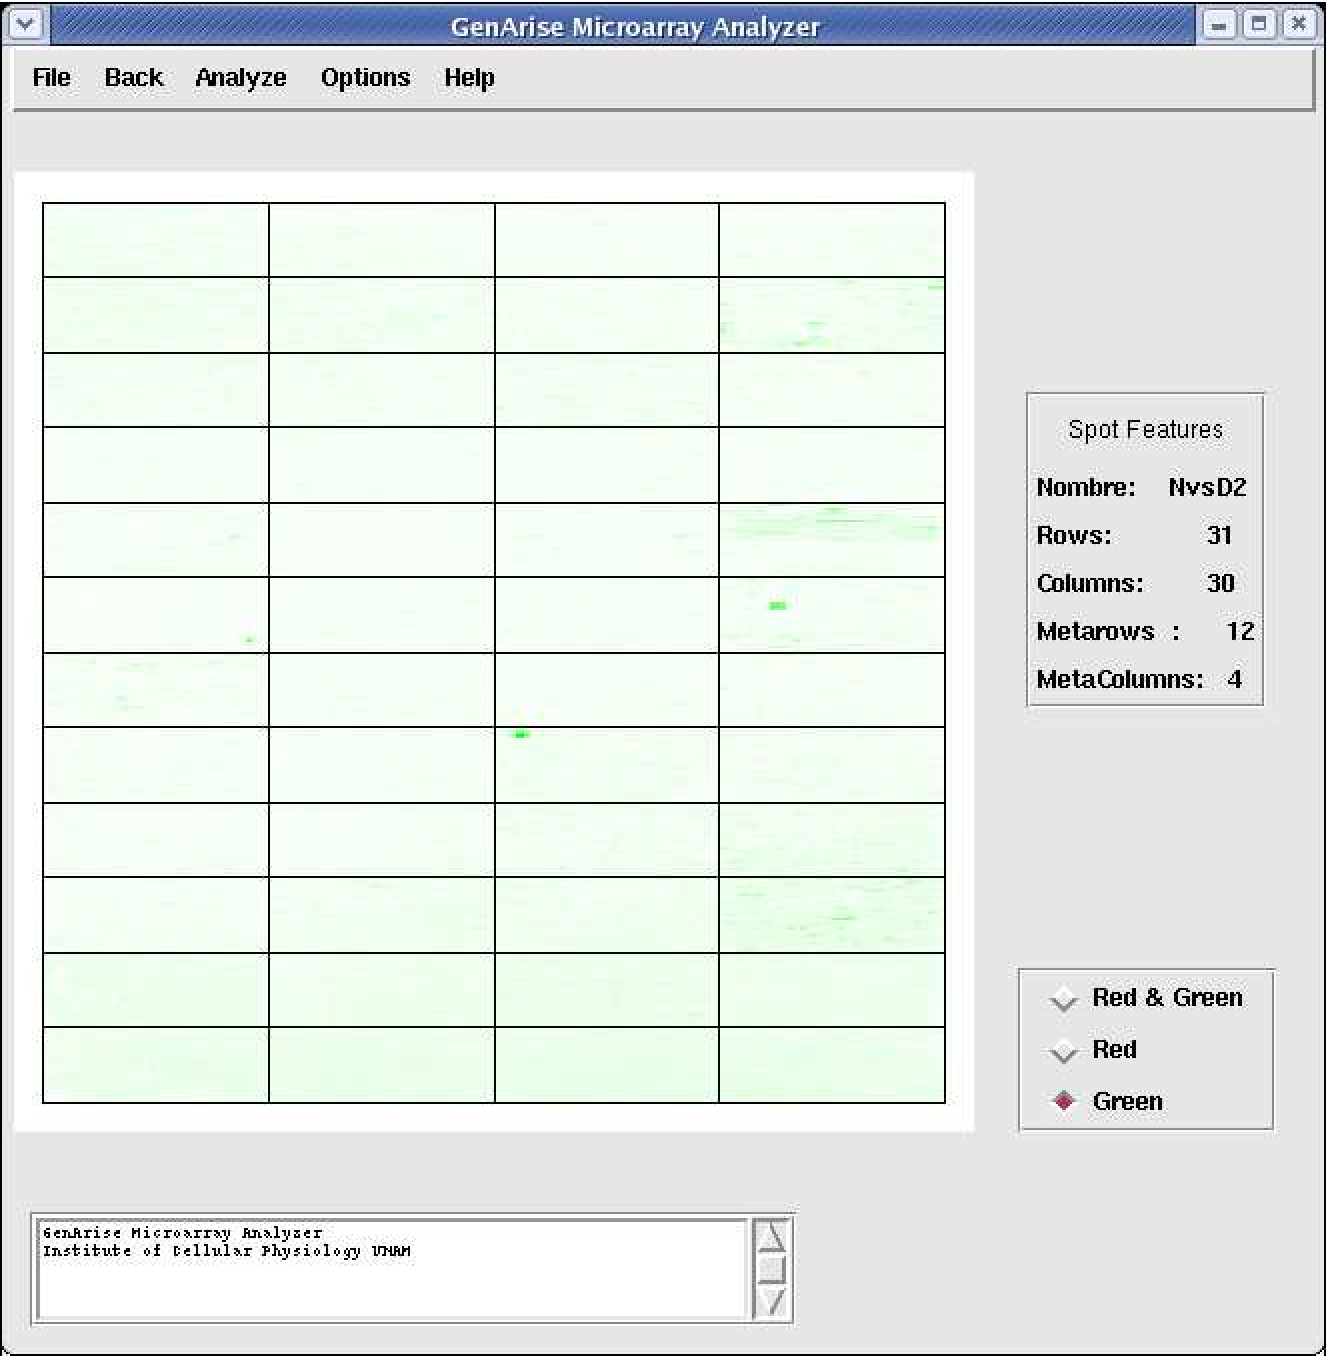
\includegraphics[height=3in,width=3.15in]{./images/principalGreen.pdf}\\
\caption{Window with image plot for Cy5 Background value. \label{fig19}}
\end{center}
\end{figure}

In the upper right side of the window we can see the data attributes of the file that is being analyzed and the experiment configuration.\\
You can save the plot in a pdf file by selecting the option \textbf{Save as PDF} in the menu Options. With the option \textbf{Annotations} of the same menu, you can make some important annotations through the analysis and save these in a file called annotations.txt. See Figure \ref{fig20}.
\begin{figure}[h]
\begin{center}
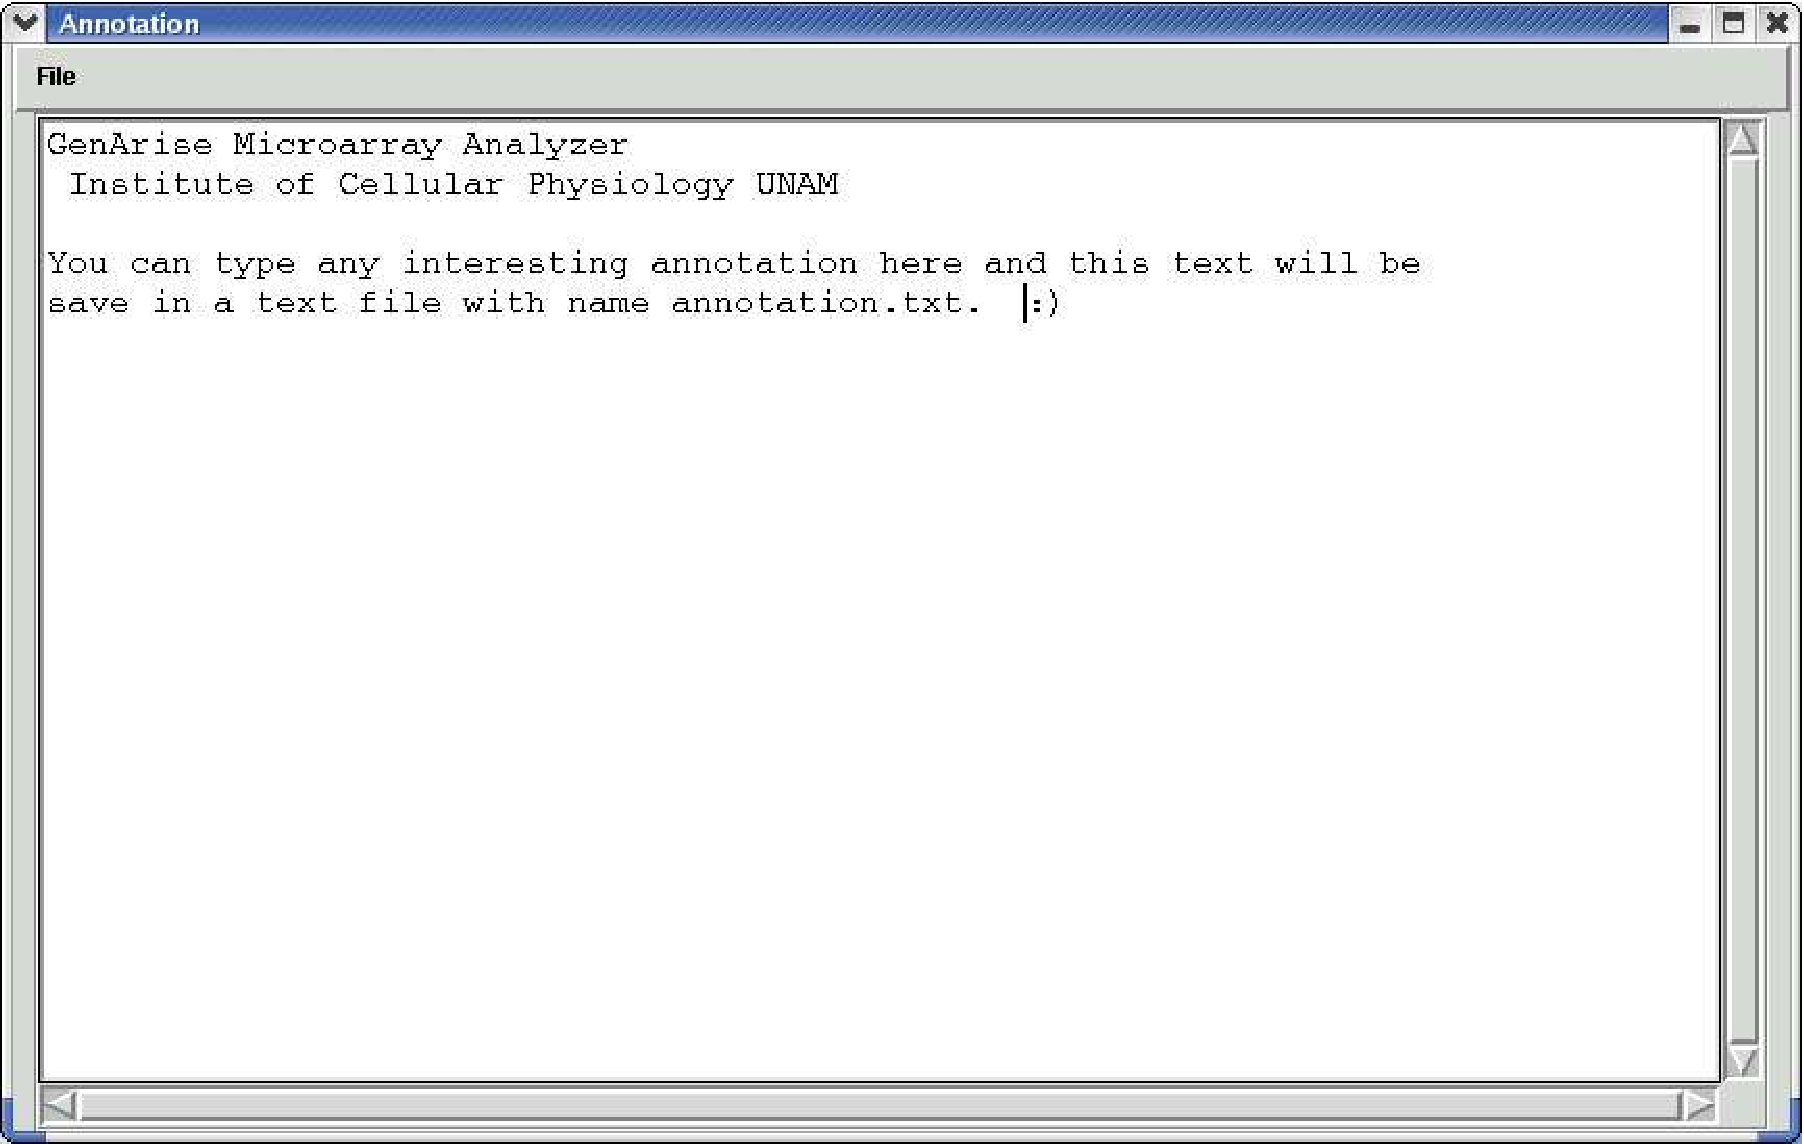
\includegraphics[scale= 0.3]{./images/annotation.pdf}\\
\caption{An Editor for annotations. \label{fig20}}
\end{center}
\end{figure}

At this moment you can begin the analysis by clicking on the menu Analyze that will display a dialog box like the one showed in Figure \ref{fig21}.\\
\begin{figure}[h]
\begin{center}

\includegraphics[scale= 0.3]{./images/wizarddialog.pdf}\\
\caption{Asking dialog box.\label{fig21}}
\end{center}
\end{figure}

By clicking \textbf{Yes }the program makes the operations in the next sequential order: background correction, loess normalization, intensity-filter, duplicate elimination. Once this analysis end we see the next window. See Figure \ref{fig22}.\\

\begin{figure}[h]
\begin{center}
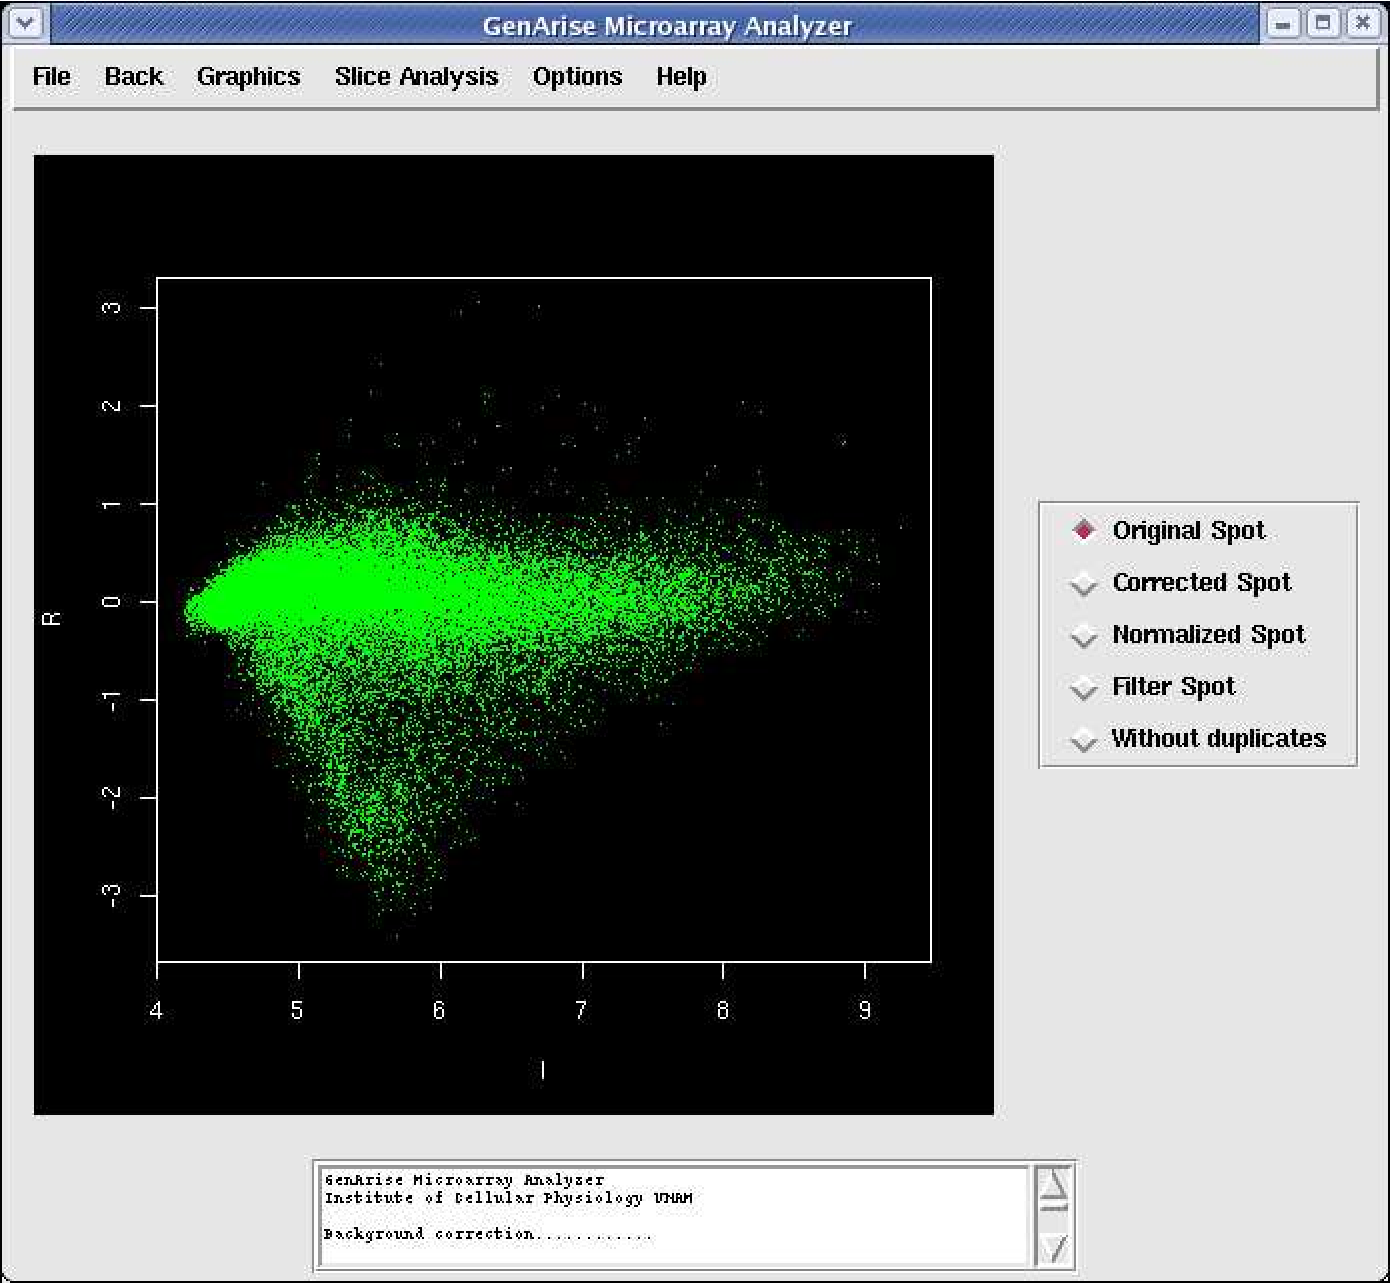
\includegraphics[scale= 0.3]{./images/wizardOriginal.pdf}\\
\caption{Text area while analysis. \label{fig22}}
\end{center}
\end{figure}

This window shows the graphic obtained from the complete analysis, also shows five options where you can select the original-experiment graphic and after each operation; for example after select the option \textbf{Normalized Spot} the next result is shown in Figure \ref{fig23}.\\
\begin{figure}[h]
\begin{center}
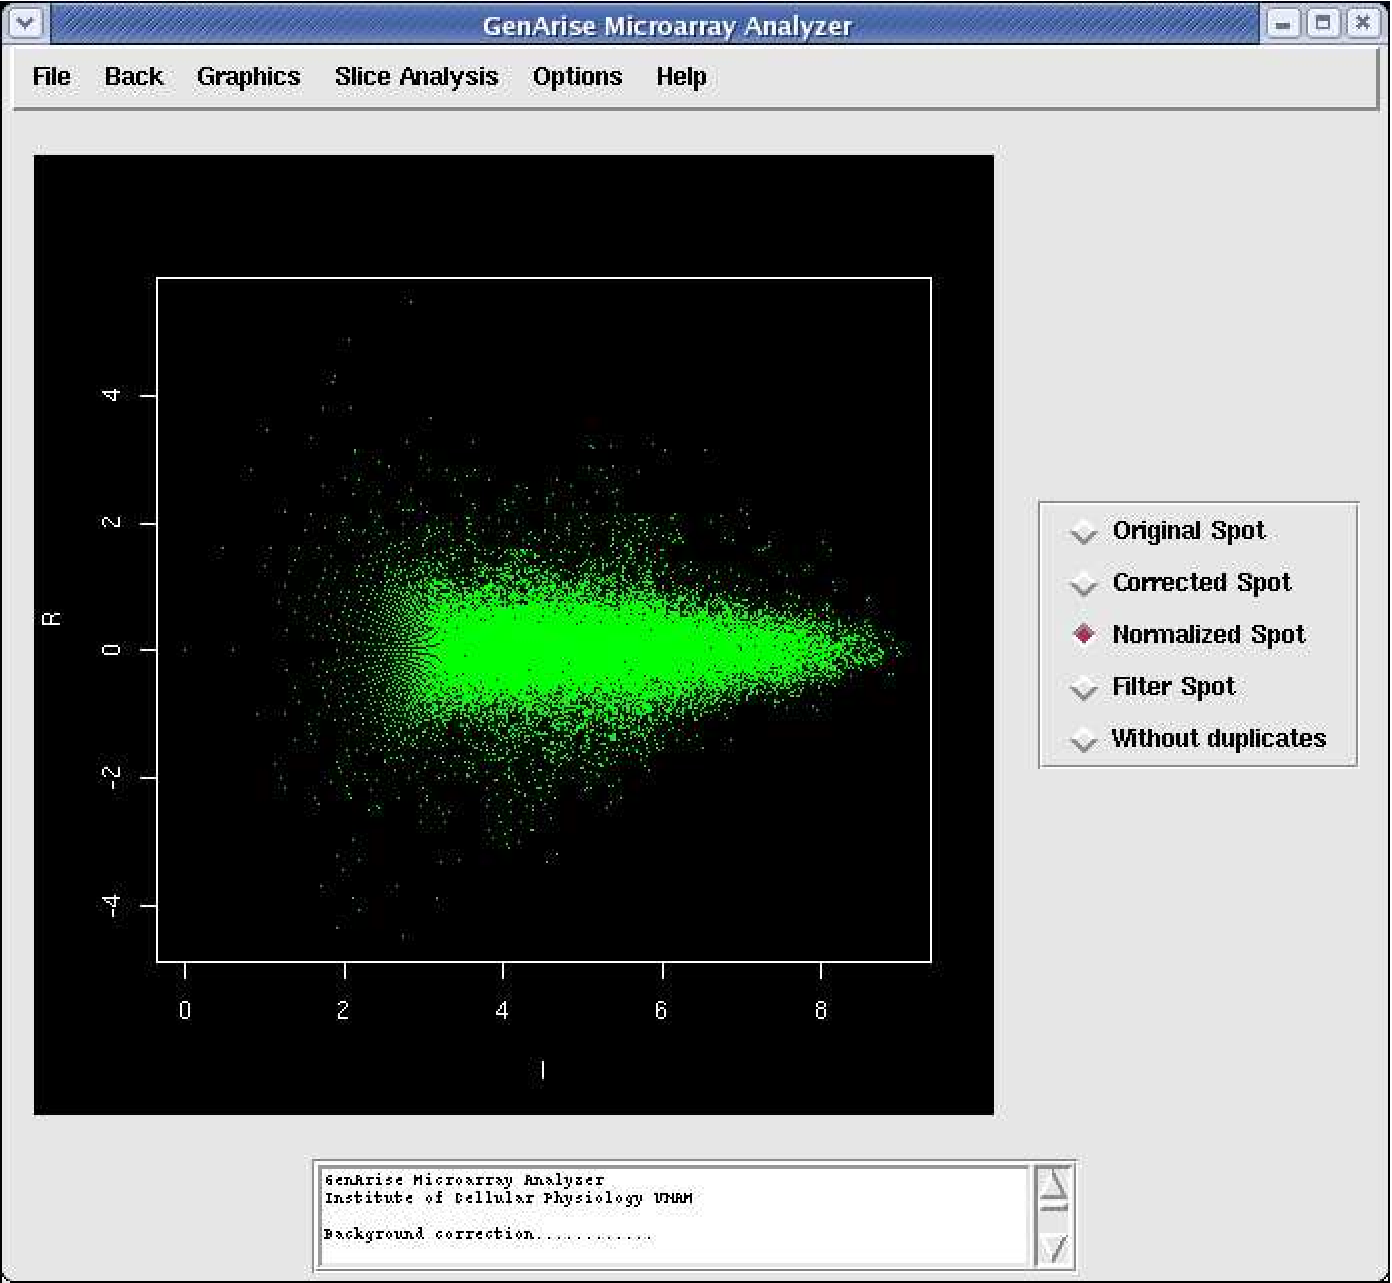
\includegraphics[scale= 0.3]{./images/wizardNorm.pdf}\\
\caption{You can select any step of this analisis for preview \label{fig23}}
\end{center}
\end{figure}

There is a text area in the lower side of the window where you can find the operations done and their values.When you follow the wizard the default values are employed in the operations. We use the grid normalization.\\
The menu \textbf{Graphics} allows you change the type of the graphic that is displayed. The options are:  \textbf{Cy3 vs Cy5, R vs I } and \textbf{M vs A}. See Figure \ref{fig24}.\\

\begin{figure}
\begin{center}
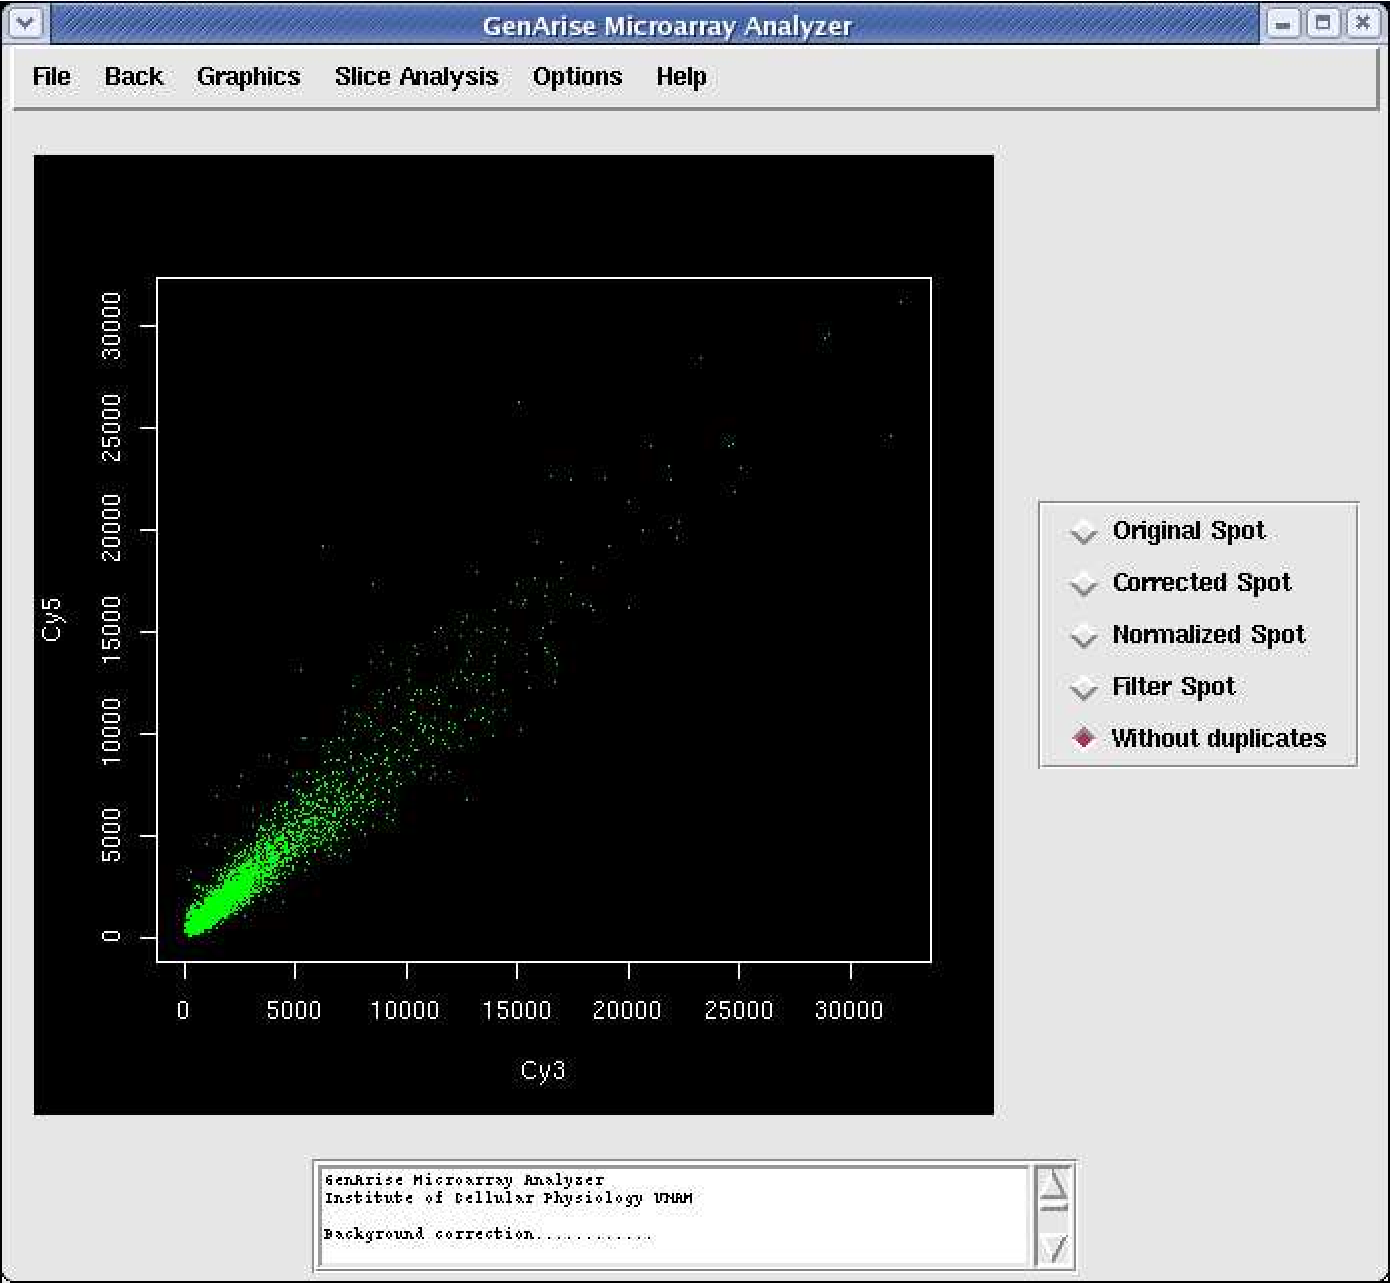
\includegraphics[scale= 0.3]{./images/nodupsCy3vsCy5.pdf}
\caption{Cy3 vs Cy5 plot \label{fig24}}
\end{center}
\end{figure}

At the end, you find one file for each operation done, as well as for each graphic, in the directory where are the result files of your project.\\

Let see what happen if you decide not to follow the wizard. In this case, only the original-experiment graphic is displayed as shown in Figure \ref{fig25}.\\

\begin{figure}
\begin{center}
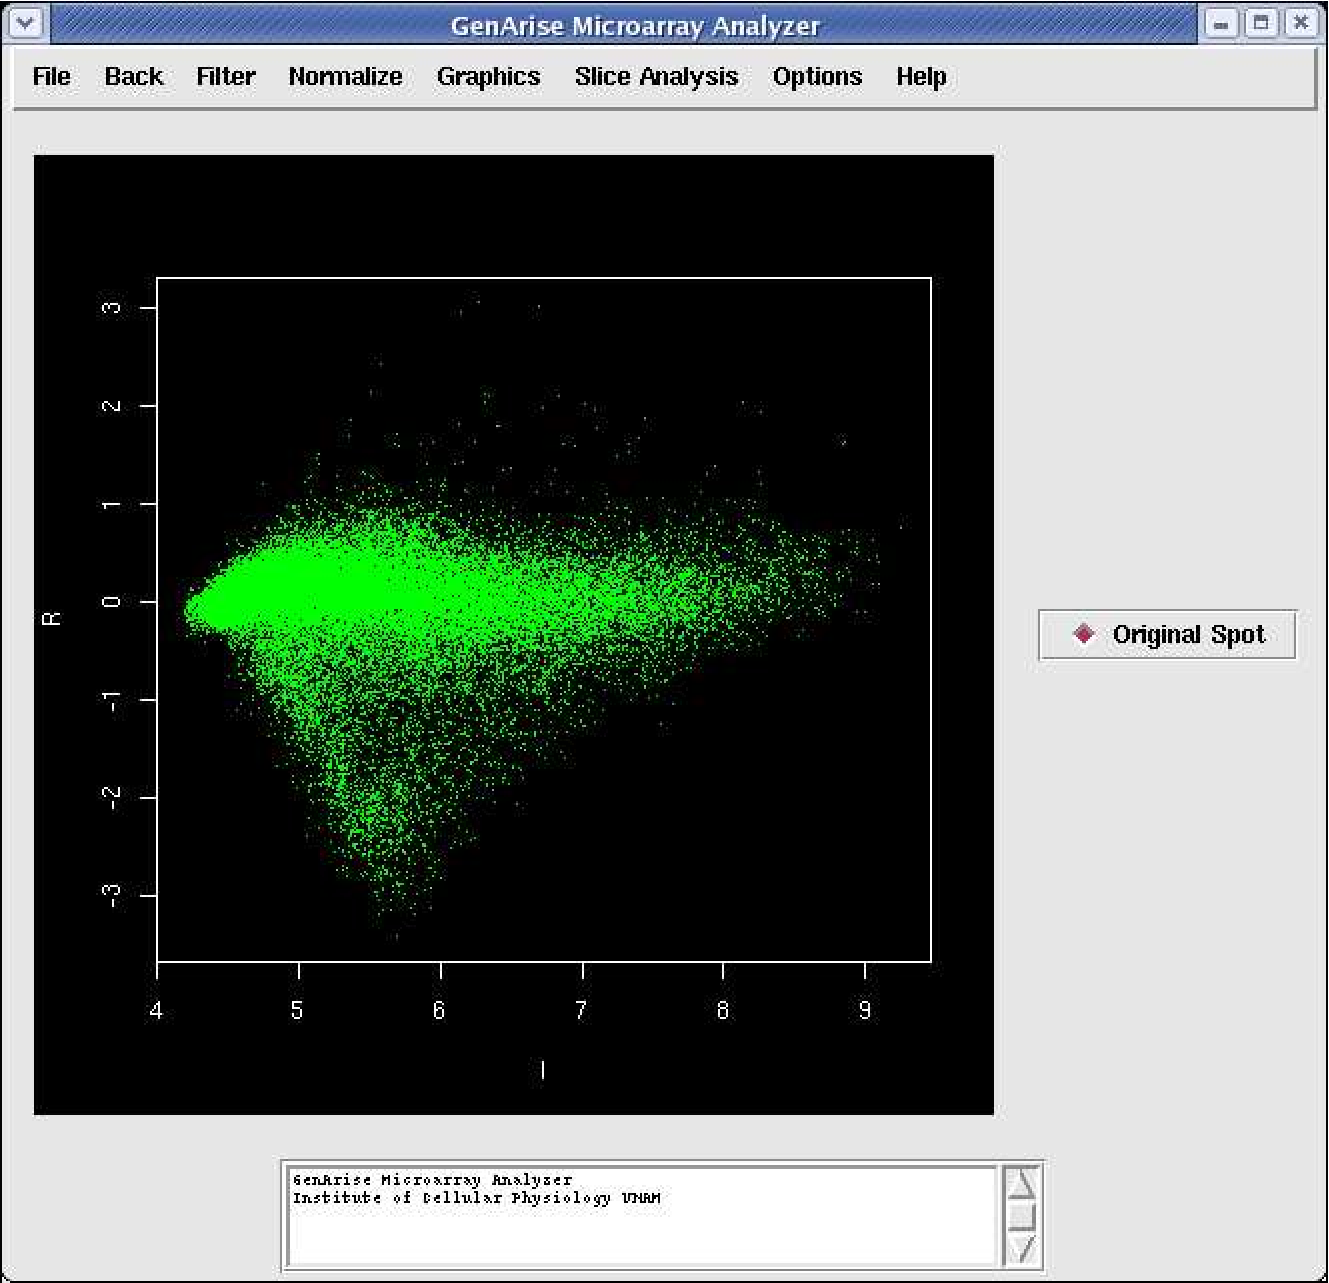
\includegraphics[scale= 0.3]{./images/original.pdf}
\caption{Making the analysis without follow the wizard. \label{fig25}}
\end{center}
\end{figure}

In the menu bar you should select the operations you wish the program make in the desired order, once an operation is made a new reference to the transformed spot will appear in the right side of the window with which you can see the graphic's results obtained with that operation. Is important to note that the operations are performed on the selected spot. If we wish to make a sequential analysis you must take care of the selected option. The operations that the program makes when you decide to follow the wizard are the same that you can find in the menu \textbf{Options}.\\

\end{document}
